\documentclass[10pt,a4paper,oneside]{article}
\usepackage[brazil]{babel}
\usepackage[utf8]{inputenc}
\usepackage{amsmath}
\usepackage{amsfonts}
\usepackage{amssymb}
\usepackage[left=3cm,right=3cm,top=2cm,bottom=2cm]{geometry}

% TODOs.
\usepackage{todonotes}

% Floats.
\usepackage{placeins}

% Captions
\usepackage{caption}
\usepackage{capt-of}
% subfigure
%\usepackage{subcaption}

\usepackage{xspace}
\usepackage{graphicx}

\newcommand{\arat}{Aratibutantã\xspace}
\newcommand{\baep}{Baependinha\xspace}
\newcommand{\itam}{Itamaracanã\xspace}
\newcommand{\jaqu}{Jaquereçaba\xspace}
\newcommand{\para}{Paranapitanga\xspace}

\newcommand{\adm}{Administração\xspace}
\newcommand{\comp}{Computação e Matemática\xspace}
\newcommand{\edu}{Educacional\xspace}
\newcommand{\eng}{Engenharia e Produção\xspace}
\newcommand{\hum}{Humanidades\xspace}
\newcommand{\jur}{Jurídica e Contábil\xspace}

% Tabelas.
\usepackage{multirow}
\usepackage{booktabs}
\newcommand{\specialcell}[3][c]
{\begin{tabular}[#1]{@{}#2@{}}#3\end{tabular}}

\author{%
	Alexis A. Huf, %
	Alyson D. Pereira, %
	Bruno C. N. Oliveira,\\%
	Eliza Gomes, %
	Pedro H. Penna
	}

\title{Lista de Exercício I - Grupo 6}


\begin{document}

\maketitle

\begin{center}
\section*{Parte 1: Pré-Análise de Dados}
\end{center}

\section{Dados Perdidos}
\label{section:dados-perdidos}

Este relatório considera dados perdidos como aqueles que não puderam ser recuperados por não estarem preenchidos. A Tabela \ref{table: dados perdidos} apresenta a quantidade de dados perdidos e seus respectivos percentuais em relação a cada variável analisada na base de dados em estudo. Constatou-se um total de 106 dados perdidos para todas as variáveis, o que representa apenas $2.12\%$ do total. Pode-se considerar, portanto, como aceitável a quantidade de dados perdidos, uma vez que está abaixo dos $5\%$ definidos como percentual aceitável.

\section{Dados Errados}
\label{section:dados-errados}

A Tabela \ref{table: dados errados} resume os erros de coleta e seus respectivos percentuais na base de dados em estudo. Além de ausência de informação, isto é, os dados perdidos analisados na seção anterior, foram evidenciados erros de ortografia, digitação e formatação (ex: espaços em branco excedentes). 

As Tabelas \ref{table: erros-regiao}, \ref{table: erros-area}, \ref{table: erros-pagamento} e \ref{table: erros-opiniao} apresentam os erros observados para as variáveis qualitativas \textit{Região}, \textit{Área}, \textit{Pagamento} e \textit{Opinião}, respectivamente.
Para as variáveis quantitativas \textit{Renda} e \textit{Idade}, não foram observados erros na base de dados, isto é, valores infactíveis (ex: \textit{Renda} não positiva e \textit{Idade} inferior a 17 ou superior a 100 anos).

Para evitar que erros de ortografia e formatação sejam cometidos nas variáveis qualitativas, pode-se utilizar um formulário de múltipla escolha de modo a evitar que as informações sejam preenchidas de maneira textual. Já para as variáveis quantitativas, no caso de um formulário eletrônico, limites inferiores e superiores de valores válidos poderiam ser checado previamente à submissão da observação. Por outro lado, quanto aos dados perdidos que não foram preenchidos, é possível criar opções de modo que as pessoas possam informar explicitamente se não sabem ou, ainda, se não desejam responder. Ademais, é possível também aplicar um teste do questionário a um grupo menor de pessoas com o objetivo de testá-lo e verificar a sua adequação, para, posteriormente, aplicá-lo a um grupo maior. Assim, problemas de entendimento podem ser resolvidos nesta fase de teste, tendendo a reduzir o percentual de erros ou informações faltantes.

\begin{figure}[h]
\begin{minipage}{0.49\textwidth}
\footnotesize
\centering
\captionof{table}{Dados perdidos na base de dados.}
\label{table: dados perdidos}
\vspace{0.5em}
\begin{tabular}{l r r}
	\toprule
	\textbf{Variável} & \textbf{\specialcell{c}{Dados\\Perdidos}} & \textbf{\specialcell{c}{Perdas\\Percentuais}} \\
	\midrule
	Área              & $21$            & $0.42\%$          \\
	Idade             & $13$            & $0.26\%$          \\
	Opinião           & $19$            & $0.38\%$          \\
	Pagamento         & $18$            & $0.36\%$          \\
	Região            & $21$            & $0.42\%$          \\
	Renda             & $14$            & $0.28\%$          \\
	\bottomrule
\end{tabular}
\end{minipage}
%
\begin{minipage}{0.49\textwidth}
\footnotesize
\centering
\captionof{table}{Erros na base de dados.}
\label{table: dados errados}
\vspace{0.5em}
\begin{tabular}{l r r}
	\toprule
	\textbf{Variável} & \textbf{\specialcell{c}{Dados\\Errados}} & \textbf{\specialcell{c}{Erros\\Percentuais}} \\
	\midrule
	Área              & $114$                                    & $2.28\%$          \\
	Idade             & $0$                                      & $0.00\%$          \\
	Opinião           & $123$                                    & $2.46\%$          \\
	Pagamento         & $132$                                    & $2.64\%$          \\
	Região            & $135$                                    & $2.71\%$          \\
	Renda             & $0$                                      & $0.00\%$          \\
	\bottomrule
\end{tabular}
\end{minipage}
\end{figure}

\begin{table}[!h]
\footnotesize
\centering
\begin{minipage}[t]{0.49\textwidth}
\caption{Erros para a variável \textit{Região}.}
\vspace{0.5em}
\label{table: erros-regiao}
\begin{tabular}{l r r}
	\toprule
	\textbf{Erro} & \textbf{Absoluto}  & \textbf{Percentual} \\
	\midrule
	Arati      & 6  & $0.12\%$ \\
	Aratib     & 12 & $0.24\%$ \\
	Aratibu    & 5  & $0.10\%$ \\
	Aratibut   & 12 & $0.24\%$ \\
	Baepe      & 17 & $0.34\%$ \\
	Baepen     & 18 & $0.36\%$ \\
	Baepend    & 12 & $0.24\%$ \\
	Baependi   & 9  & $0.18\%$ \\
	Itama      & 5  & $0.10\%$ \\
	Itamar     & 6  & $0.12\%$ \\
	Itamara    & 3  & $0.06\%$ \\
	Itamarac   & 7  & $0.14\%$ \\
	Jaque      & 5  & $0.10\%$ \\
	Jaquer     & 10 & $0.20\%$ \\
	Jaquere    & 5  & $0.10\%$ \\
	Jaquereç   & 3  & $0.06\%$ \\
	\midrule
	\textbf{Total de erros}  & 135  & $2.71\%$ \\	
	\bottomrule
\end{tabular}
\end{minipage}
%
\begin{minipage}[t]{0.49\textwidth}
\footnotesize
\caption{Erros para a variável \textit{Área}.}
\vspace{0.5em}
\label{table: erros-area}
\begin{tabular}{l r r}
	\toprule
	\textbf{Erro} & \textbf{Absoluto}  & \textbf{Percentual} \\
	\midrule
	Admin      & 3   & $0.06\%$ \\
	Admini 	   & 3   & $0.06\%$ \\
	Adminis    & 2   & $0.04\%$ \\
	Administ   & 5   & $0.10\%$ \\
	Compu      & 1   & $0.02\%$ \\
	Comput     & 2   & $0.04\%$ \\
	Computa    & 2   & $0.04\%$ \\
	Computaç   & 1   & $0.02\%$ \\
	Educa      & 2   & $0.04\%$ \\
	Educac     & 2   & $0.04\%$ \\
	Educaci    & 1   & $0.02\%$ \\
	Educacio   & 1   & $0.02\%$ \\
	Engen      & 15  & $0.30\%$ \\
	Engenh     & 9   & $0.18\%$ \\
	Engenha    & 8   & $0.16\%$ \\
	Engenhar   & 14  & $0.28\%$ \\
	Human      & 3   & $0.06\%$ \\
	Humani     & 3   & $0.06\%$ \\
	Humanid    & 4   & $0.08\%$ \\
	Humanida   & 5   & $0.10\%$ \\
	Juríd      & 3   & $0.06\%$ \\
	Jurídi     & 7   & $0.14\%$ \\
	Jurídic    & 11  & $0.22\%$ \\
	Jurídica   & 7   & $0.14\%$ \\	
	\midrule
	\textbf{Total de erros}  & 114  & $2.28\%$ \\	
	\bottomrule
\end{tabular}
\end{minipage}
\end{table}

\begin{table}[!h]
\footnotesize
\centering
\begin{minipage}[t]{0.49\textwidth}
\caption{Erros para a variável \textit{Pagamento}.}
\vspace{0.5em}
\label{table: erros-pagamento}
\begin{tabular}{l r r}
	\toprule
	\textbf{Erro} & \textbf{Absoluto}  & \textbf{Percentual} \\
	\midrule
	Auxíl     		& 3   & $0.06\%$ \\
	Auxíli 	  		& 2   & $0.04\%$ \\
	Auxílio    	 	& 2   & $0.04\%$ \\
	Auxílio \textit{(espaço)}   	& 1   & $0.02\%$ \\
	Bolsa      	 	& 3   & $0.06\%$ \\
	Bolsas     	 	& 1   & $0.02\%$ \\
	Bolsas d   	 	& 5   & $0.10\%$ \\
	Finan      	 	& 15  & $0.30\%$ \\
	Financ     	 	& 13  & $0.26\%$ \\
	Financi    	 	& 19  & $0.38\%$ \\
	Financia   	 	& 13  & $0.26\%$ \\
	Incen      	 	& 8   & $0.16\%$ \\
	Incent     	 	& 11  & $0.22\%$ \\
	Incenti    	 	& 11  & $0.22\%$ \\
	Incentiv   	 	& 10  & $0.20\%$ \\
	Recur      	 	& 4   & $0.08\%$ \\
	Recurs     	 	& 4   & $0.08\%$ \\
	Recurso    	 	& 5   & $0.10\%$ \\
	Recursos   	 	& 2   & $0.04\%$ \\	
	\midrule
	\textbf{Total de erros}  & 132  & $2.64\%$ \\	
	\bottomrule
\end{tabular}
\end{minipage}
%
\begin{minipage}[t]{0.49\textwidth}
\footnotesize
\caption{Erros para a variável \textit{Opinião}.}
\vspace{0.5em}
\label{table: erros-opiniao}
\begin{tabular}{l r r}
	\toprule
	\textbf{Erro} & \textbf{Absoluto}  & \textbf{Percentual} \\
	\midrule
	Indifer    & 14  & $0.28\%$ \\
	Indifere   & 16  & $0.32\%$ \\
	Insatis    & 7   & $0.14\%$ \\
	Insatisf   & 10  & $0.20\%$ \\
	Muito i    & 3   & $0.06\%$ \\
	Muito in   & 5   & $0.10\%$ \\
	Muito s    & 22  & $0.44\%$ \\
	Muito sa   & 28  & $0.56\%$ \\
	Satisfe    & 10  & $0.20\%$ \\
	Satisfei   & 8   & $0.16\%$ \\	
	\midrule
	\textbf{Total de erros}  & 123  & $2.46\%$ \\	
	\bottomrule
\end{tabular}
\end{minipage}
\end{table}


\begin{table}[!h]
\centering

\end{table}

\FloatBarrier
\clearpage
\begin{center}
\section*{Parte 2: Análise Individual das Variáveis}
\end{center}

\section{Variável \textit{Região}}
\label{section:regiao}

A tabela frequências para a variável \textit{Região} é apresentada na Tabela \ref{table: frequencias regiao}. A análise indica que as regiões com menor e maior número de alunos são as regiões \textit{\para} e \textit{\baep}, respectivamente. Já as demais regiões apresentam um corpo discente que varia de $10.77\%$ a $23.80\%$.

\begin{table}[h]
\footnotesize
\centering
\caption{Frequências para a variável \textit{Região}}
\label{table: frequencias regiao}
\vspace{0.5em}
\begin{tabular}{l r r}
	\toprule
	\textbf{Região} & \textbf{Ocorrências} & \textbf{Frequência} \\
	\midrule
	\arat           & $1185$               & $23.80\%$           \\
	\baep           & $2294$               & $46.07\%$           \\
	\itam           & $843$                & $16.93\%$           \\
	\jaqu           & $536$                & $10.77\%$           \\
	\para           & $121$                & $2.43\%$            \\
	\bottomrule
\end{tabular}
\end{table}

\section{Variável \textit{Área}}
\label{section:area}

A tabela de frequências para a variável \textit{Área} é apresentada na Tabela \ref{table: frequencias area}. O perfil da TYU modificou-se. A análise indica que a área com o maior contingente de alunos é \textit{\eng}, na amostra atual.

\begin{table}[h]
\footnotesize
\centering
\caption{Frequências para a variável \textit{Área}}
\label{table: frequencias area}
\vspace{0.5em}
\begin{tabular}{l r r}
	\toprule
	\textbf{Área} & \textbf{Ocorrências} & \textbf{Frequência} \\
	\midrule
	\adm            & $592$                & $11.89\%$           \\
	\comp           & $296$                & $5.94\%$            \\
	\edu            & $338$                & $6.79\%$            \\
	\eng            & $1741$               & $34.97\%$           \\
	\hum            & $503$                & $10.10\%$           \\
	\jur            & $1509$               & $30.31\%$           \\
	\bottomrule
\end{tabular}
\end{table}

\section{Variável \textit{Pagamento}}
\label{section:pagamento}

A tabela de frequências para a variável \textit{Pagamento} á apresentada na Tabela \ref{table: frequencias pagamento}. A análise indica que os recursos usados para pagar as mensalidades do curso são oriundos, em sua maioria, de \textit{Financiamento Bancário} ($43.98\%$) seguido por \textit{Incentivos Federais} ($29.06\%$), somando um total de $73.04\%$. Portanto, cortes no orçamento federal de Pindorama não afetarão a fonte de recursos primária para pagamentos de mensalidades na TYU.

\begin{table}[h]
\footnotesize
\centering
\caption{Frequências para a variável \textit{Pagamento}}
\label{table: frequencias pagamento}
\vspace{0.5em}
\begin{tabular}{l r r}
	\toprule
	\textbf{Pagamento}     & \textbf{Ocorrências} & \textbf{Frequência} \\
	\midrule
	Auxilio Familiar       & $257$                & $5.16\%$            \\
	Bolsas                 & $328$                & $6.58\%$            \\
	Financiamento Bancário & $2191$               & $43.98\%$           \\
	Incentivos Federais    & $1448$               & $29.06\%$           \\
	Recursos Próprios      & $758$                & $15.21\%$           \\
	\bottomrule
\end{tabular}
\end{table}

\clearpage
\section{Variável \textit{Opinião}}
\label{section:opiniao}

A tabela de frequências para a variável \textit{Opinião} é apresentada na Tabela \ref{table: frequencias opiniao}. A análise indica que opinião predominante na amostra é \textit{Muito Satisfeito} e que o grupo de alunos que mencionaram estarem \textit{Muito satisfeito} ou \textit{Satisfeito} totaliza $55.29\%$. Portanto, pode-se considerar que a maioria dos alunos da TYU estão satisfeitos com a EAD.

\begin{table}[h]
\footnotesize
\centering
\caption{Frequências para a variável \textit{Opinião}}
\label{table: frequencias opiniao}
\vspace{0.5em}
\begin{tabular}{l r r}
	\toprule
	\textbf{Pagamento}     & \textbf{Ocorrências} & \textbf{Frequência} \\
	\midrule
	Muito Insatisfeito     & $472$                & $9.48\%$            \\
	Insatisfeito           & $749$                & $15.04\%$           \\
	Indiferente            & $1006$               & $20.20\%$           \\
	Satisfeito             & $1035$               & $20.78\%$           \\
	Muito Satisfeito       & $1719$               & $34.51\%$           \\
	\bottomrule
\end{tabular}
\end{table}

\section{Variável \textit{Renda}}
\label{section:renda}

Medidas de síntese para a variável \textit{Renda} são apresentadas na Tabela \ref{table: medidas sintese renda}. Além disso, um histograma da variável renda e um boxplot são apresentados na Figura \ref{figure:histograma-boxplot-renda}. Um desafio para a construção  de um histograma é a presença de valores discrepantes de grande magnitude. Desse modo o intervalo que abrange os valores discrepantes, $[4224, \infty)$ consiste de uma única classe no histograma. O intervalo de valores não discrepantes, $[880, 4224)$, foi dividido em 19 classes ($k = 5 \times log_{10}(4689)$), cada uma com um intervalo de $R\$ 176$.  Vale ressaltar que, para fins de estudo, aplicou-se uma transformação nessa variável, utilizando como fator multiplicativo o valor de $R\$880$ (referência salarial em Pindorama).

A análise indica que pelo menos três quartos dos alunos de EAD da TYU ainda mantém renda familiar inferior a $R\$2450.00$, uma vez que o quartil superior da amostra para essa variável é de $R$\$$2402.40$. Além disso constata-se que a distribuição da variável segue uma curva leptocúrtica (curtose $> 0$), possui assimetria à direita (assimetria $> 0$) e dispersão de $76\%$ em relação à média. Com relação aos valores discrepantes, observa-se que o conjunto de dados analisados e disponíveis na base de dados contempla $296$ valores de renda acima de R\$ $4224.00$.

\begin{figure}[h]
\centering
\begin{minipage}{0.54\textwidth}
	\centering
		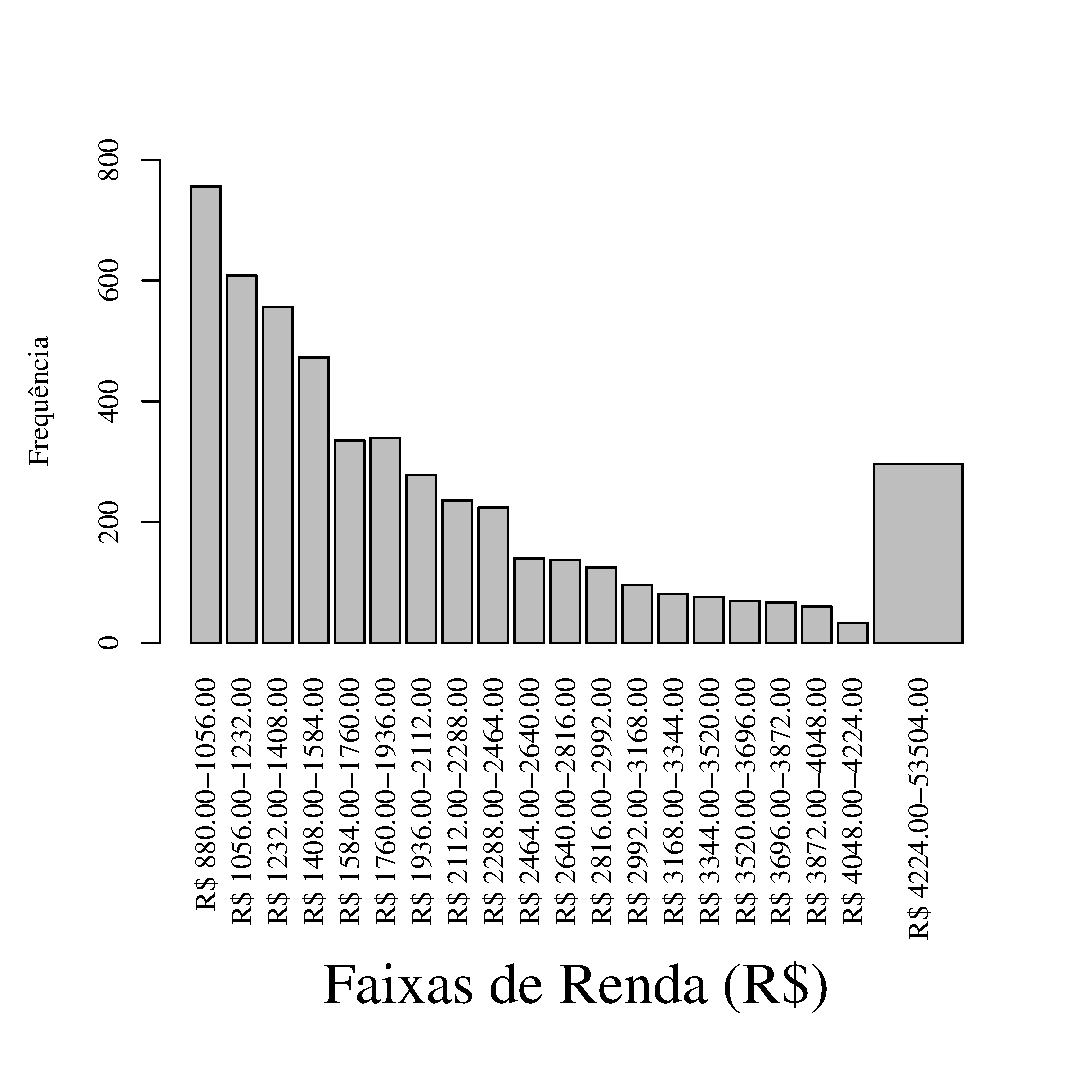
\includegraphics[width=\linewidth]{plots/histogram_renda.eps}
	\captionof{figure}{Histograma da varável \textit{Renda}.}
	\label{figure:histograma-boxplot-renda}
\end{minipage}
%
\begin{minipage}{0.44\textwidth}
	\centering
		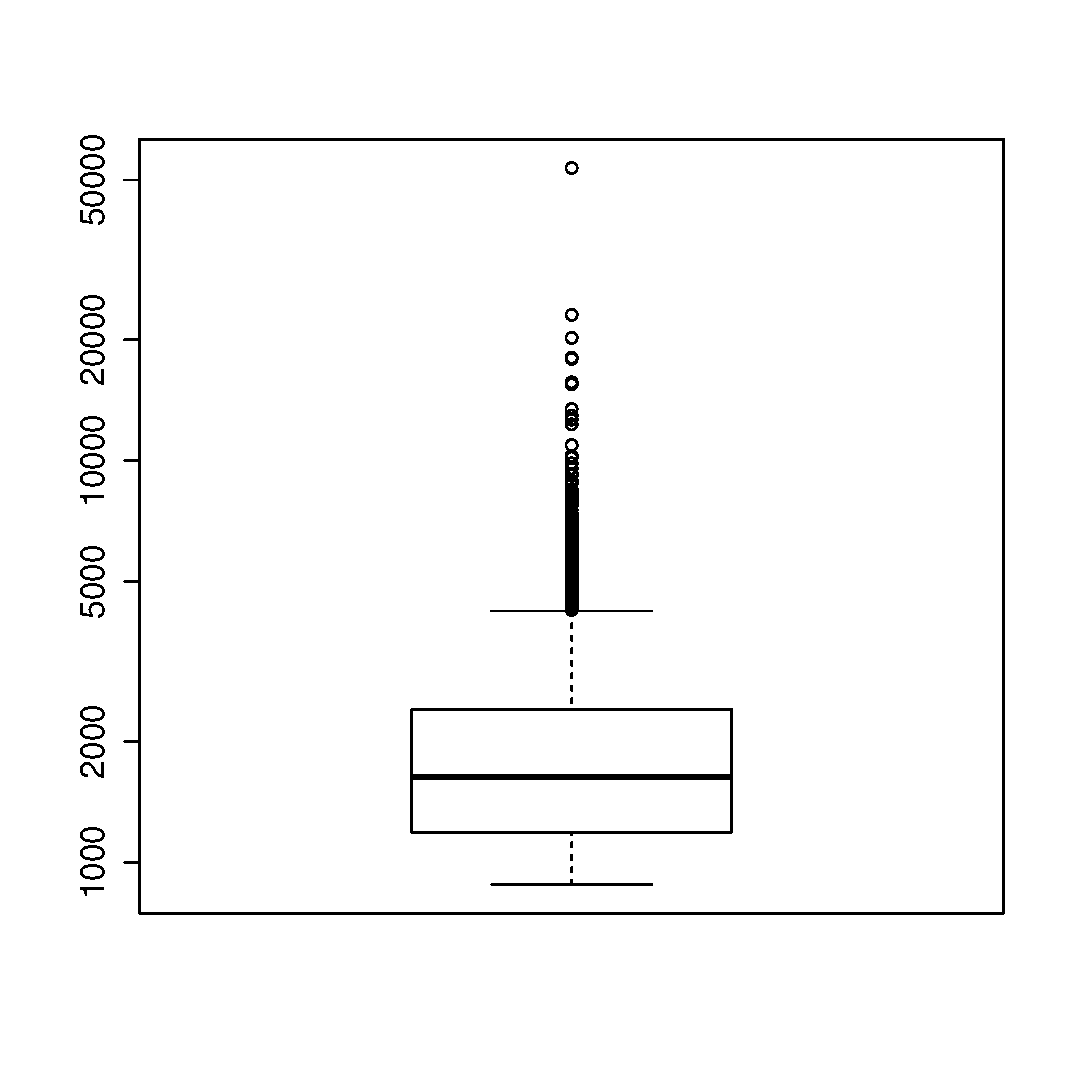
\includegraphics[width=\linewidth]{plots/boxplot_renda_log.eps}
	\captionof{figure}{\textit{Boxplot} da varável \textit{Renda}.}
	\label{figure:histograma-boxplot-renda}
\end{minipage}
\end{figure}

\begin{figure}
\centering
\begin{minipage}{0.49\textwidth}
\centering
\footnotesize
\captionof{table}{Medidas de síntese para \textit{Renda}.}
\vspace{0.5em}
\label{table: medidas sintese renda}
\begin{tabular}{l r}
	\toprule
	\textbf{Medida}               & \textbf{Renda}    \\
	\midrule
	Média                         &  R\$ $2056.05$    \\
	Moda                          &  R\$ $906.40$     \\
	Mediana                       &  R\$ $1628.00$    \\
	Variância                     &  R\$ $2449929.23$ \\
	Desvio Padrão                 &  R\$ $1565.38$    \\
	Coeficiente de Variação       &  $76\%$           \\
	Assimetria                    &  $9.94$           \\
	Curtose                       &  $253.91$         \\
	Mínimo                        &  R\$ $880.00$     \\
	Máximo                        &  R\$ $53504.00$   \\
	Quartil Inferior (Qi)         &  R\$ $1188.00$    \\
	Quartil Superior (Qs)         &  R\$ $2402.40$    \\
	Diferença Interquartil        &  R\$ $1214.40$    \\
	$Qi-1.5x(Qs-Qi)$              &  R\$ ${-633.60}$  \\
	$Qs+1.5x(Qs-Qi)$              &  R\$ $4224.00$    \\
	Dados Totais                  &  $5000$           \\
	Dados Válidos                 &  $4986$           \\
	Dados Perdidos                &  $14$             \\
	Dados Discrepantes            &  $296$            \\
	\bottomrule
\end{tabular}
\end{minipage}
%
\begin{minipage}{0.49\textwidth}
\centering
\footnotesize
\captionof{table}{Medidas de síntese para \textit{Idade}.}
\vspace{0.5em}
\label{table: medidas sintese idade}
\begin{tabular}{l r}
	\toprule
	\textbf{Medida}               & \textbf{Idade} \\
	\midrule
	Média                         & $32.18$ anos   \\
	Moda                          & $32.00$ anos   \\
	Mediana                       & $32$ anos      \\
	Variância                     & $31.83$ anos   \\
	Desvio Padrão                 & $5.64$ anos    \\
	Coeficiente de Variação       & $18 \%$        \\
	Assimetria                    & $1.205$        \\
	Curtose                       & $6.19$         \\
	Mínimo                        & $18$ anos      \\
	Máximo                        & $70$ anos      \\
	Quartil Inferior (Qi)         & $29$ anos      \\
	Quartil Superior (Qs)         & $35$ anos      \\
	Diferença Interquartil        & $6$  anos      \\
	$Qi-1.5x(Qs-Qi)$              & $20$ anos      \\
	$Qs+1.5x(Qs-Qi)$              & $44$ anos      \\
	Dados Totais                  & $5000$         \\
	Dados Válidos                 & $4987$         \\
	Dados Perdidos                & $13$           \\
	Dados Discrepantes            & $98$           \\
	\bottomrule
\end{tabular}
\end{minipage}
\end{figure}

\FloatBarrier
\section{Variável \textit{Idade}}
\label{section:idade}

Medidas de síntese para a variável \textit{Idade} são apresentadas na Tabela \ref{table: medidas sintese idade}. Além disso, um histograma da variável idade é apresentado na Figura \ref{figure:histograma-boxplot-idade}.

A análise indica que a maioria dos alunos de EAD na TYU possuem mais de $30$ anos. Essa conclusão pode ser tomada com base mediana, que assume valor $32$ anos. Mais especificamente, a proporção de alunos com mais de 30 anos na amostra é de $61.4\%$. Fazendo uma comparação com o perfil antigo, pode-se afirmar que o perfil dos alunos mudou, agora a maioria dos alunos são dois anos mais velhos, de $30$ para $32$ anos.

Fazendo uma análise mais detalhada da variável em estudo, percebe-se que ela segue uma distribuição com curtose leptocúrtica (curtose $> 0$), assimetria positiva (assimetria $> 0$) e dispersão de $18\%$ em relação à média. Além disso, podemos observar que pelo quartil inferior e superior, que $50\%$  dos alunos possuem de $29$ a $35$ anos. Vale observar, que dos $98$ valores discrepantes na amostra, a maioria ($69$ observações) encontram-se superiores a $44$ anos.

\begin{figure}[h]
\centering
\begin{minipage}{0.54\textwidth}
	\centering
	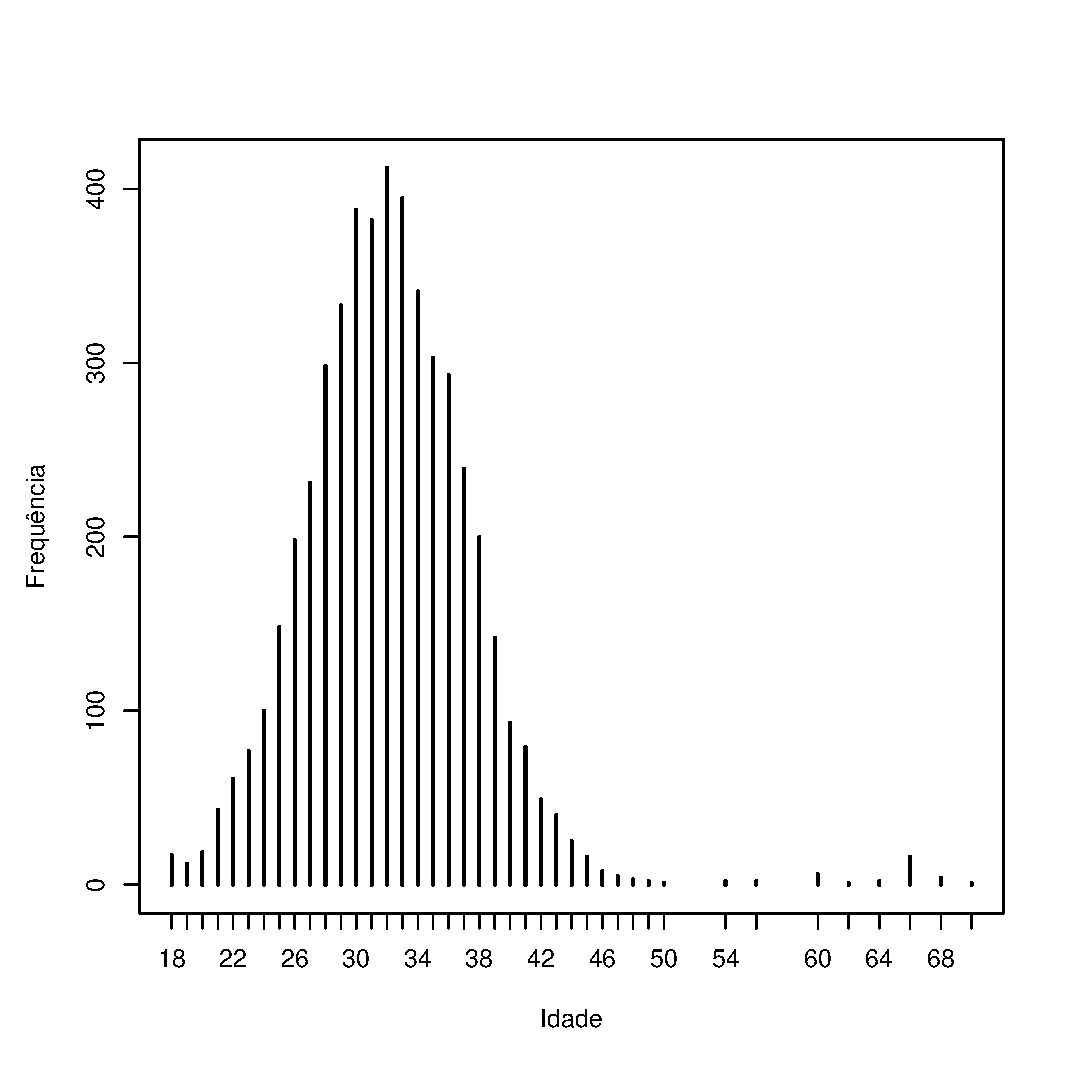
\includegraphics[width=\linewidth]{plots/histogram_idade_log.eps}
	\caption{Histograma da variável \textit{Idade}.}
	\label{figure:histograma-boxplot-idade}
\end{minipage}
%
\begin{minipage}{0.44\textwidth}
	\centering
	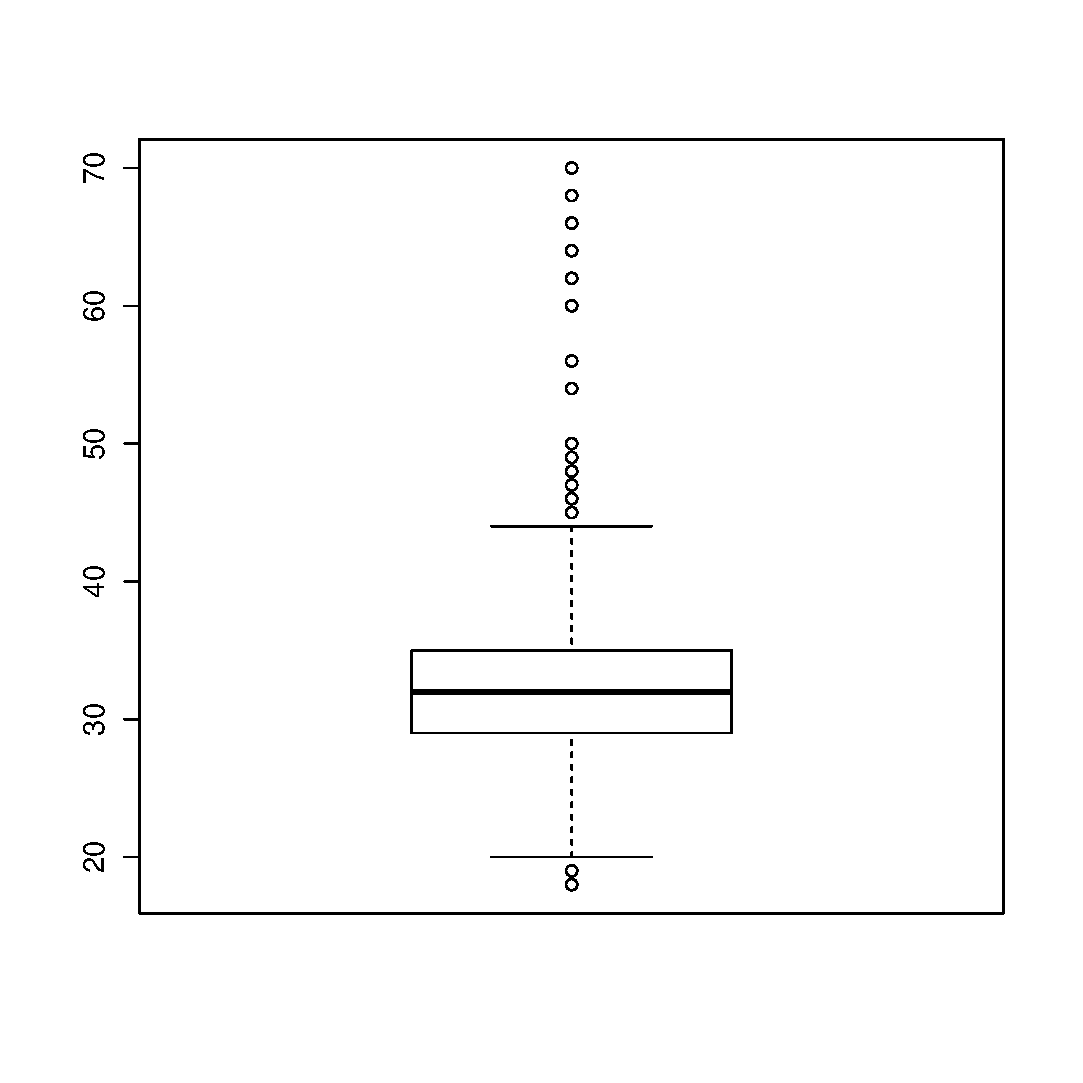
\includegraphics[width=\linewidth]{plots/boxplot_idade.eps}
	\caption{\textit{Boxplot} da variável \textit{Idade}.}
	\label{figure:histograma-boxplot-idade}
\end{minipage}
\end{figure}

\FloatBarrier
\clearpage
\begin{center}
\section*{Parte 3: Análise em Conjunto de Duas Variáveis}
\end{center}

\section{Opinião por Região}
\label{section:opiniao-regiao}

A Tabela \ref{table:satisfacao-regiao} apresenta uma análise da variável \textit{Opinião} agrupada por \textit{Região}. Registros com valores faltantes em qualquer uma das duas variáveis foram desconsiderados. Identificando as opiniões que compõem mais de 50\% da amostra para cada região, conclui-se que o perfil atual se difere do antigo. Para as regiões \jaqu e \para, observou-se que a avaliação dos alunos piorou. Já para as demais regiões, percebeu-se uma melhoria na avaliação. 

Vale ressaltar que na avaliação atual, $55.29\%$ dos alunos estão satisfeitos ou muito satisfeitos. No entanto, os \textit{campi} que concentram as maiores taxas de insatisfação, (\arat e \para), contém apenas $26.12\%$ dos alunos. Adicionalmente, \baep, onde os alunos estão majoritariamente satisfeitos ou muito satisfeitos, concentra $45.88\%$ dos 5000 alunos. O gráfico da Figura \ref{fig:stacked-opiniao-por-regiao} mostra visualmente como \baep e \itam mascaram o péssimo resultado de \arat e \para quando a amostra inteira é considerada.

\begin{table}[!h]
	\footnotesize
	\centering
	\caption{Satisfação por região.}
	\label{table:satisfacao-regiao}
	\begin{tabular}{l l l}
		\toprule
		\textbf{Região} & \textbf{Avaliação Antiga} & \textbf{Avaliação Atual}                \\
		\midrule
		\arat  & Muito Insatisfeito & Indiferente ($38.48\%$) e Insatisfeito ($32.15\%$)      \\
		\baep  & Muito Insatisfeito & Satisfeito ($33.96\%$) e Muito Satisfeito ($38.19\%$)   \\
		\itam  & Satisfeito         & Muito Satisfeito ($93.94\%$)                            \\
		\jaqu  & Indiferentes       & Insatisfeito ($33.93\%$) e Muito Insatisfeito ($44.03\%$) \\
		\para  & Diversas           & Muito Insatisfeito ($91.74\%$)                          \\
		\bottomrule
	\end{tabular}
\end{table}
\vspace{-4em}
\begin{figure}[!h]
	\centering
	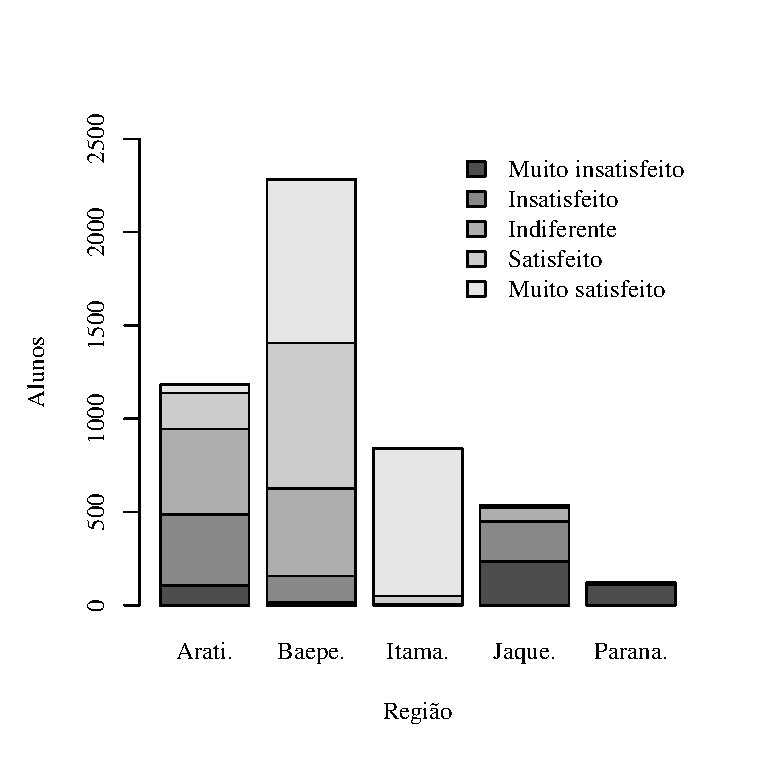
\includegraphics[scale=0.70]{plots/stacked_opiniao_por_regiao.eps}
	\caption{Gráfico empilhado de opinião para cada região.}
	\label{fig:stacked-opiniao-por-regiao}
\end{figure}

\FloatBarrier
\section{Opinião por Área}
\label{section:opiniao-area}

De um modo geral, o investimento resultou em uma melhora na avaliação dos cursos \edu, \hum e \eng, e estabilidade na avaliação para os cursos de \comp e \adm. Portanto, o investimento foi eficaz. A Tabela \ref{table:opiniao-por-area} mostra a distribuição da opinião dos alunos para cada área do conhecimento, enquanto a Figura \ref{fig:stacked-opiniao-por-area} apresenta os mesmos dados em um gráfico empilhado usando valores absolutos da quantidade de alunos. Tanto na figura quanto na tabela, amostras sem valor para a variável \textit{Opinião} ou para a variável \textit{Área} foram desconsiderados no cálculo do percentual. Para análise da variável \textit{Opinião} agrupada por \textit{Área}, registros com valores faltantes em qualquer uma das duas variáveis foram igualmente desconsiderados.

Na avaliação antiga, os alunos dos cursos das áreas \edu e de \hum estavam muito insatisfeitos. Atualmente, $89.91\%$ dos alunos da área \edu estão muito satisfeitos e $74.9\%$ dos alunos de \hum estão muitos satisfeitos. Considerando os alunos que se disseram muito satisfeitos ou apenas satisfeitos com o curso, estes correspondem a $97.63\%$ dos cursos da área \edu e a $91.63\%$ da área \hum.

Na avaliação antiga dos cursos de \comp e de \adm, os alunos elogiaram seus cursos, mantendo esta carcterística atualmente. Para os cursos de \comp e \adm, $75.26\%$ e $85.09\%$ dos alunos reportaram estarem satisfeitos ou muito satisfeitos, respectivamente.

Na avaliação antiga os alunos de cursos das demais áreas (\eng e \jur) tinham opinião majoritariamente indiferente. Todavia, esta característica foi alterada na recente pesquisa. A quantidade de alunos satisfeitos ou muito satisfeitos nos cursos de \eng corresponde a um total de $53.82\%$, enquanto o percentual de alunos indiferentes é de $27.89\%$, indicando uma melhora. Já para o curso de Jurídica e Contábil, o percentual de alunos insatisfeitos ou muito insatisfeitos é alto, correspondendo a um total de $56.62\%$ do total de alunos do curso, com $23.65\%$ indiferentes e apenas $19.74\%$ satisfeitos ou muito satisfeitos. Os cursos da área  \jur apresentaram uma deterioração no período e devem receber atenção especial. A urgência da tomada de ações para melhorar a opinião dos alunos da área \jur é agravada pelo grande número de alunos nessa área, correspondendo a  $30.18\%$ do total de 5000 alunos na amostra.

\begin{table}[!h]
	\footnotesize
	\centering
	\caption{Opinião por área do conhecimento}
	\label{table:opiniao-por-area}
	\begin{tabular}{l r r r r r}
		\toprule
		\textbf{Curso}                   & \textbf{\specialcell{c}{Muito\\Insatisfeito}} & \textbf{Insatisfeito} &  \textbf{Indiferente} &  \textbf{Satisfeito} & \textbf{\specialcell{c}{Muito\\Satisfeito}} \\
		\midrule
		%                        Muito Ins  & Insatisfeito  & Indiferente & Satisfeito & Muito Satis           
		Administração           & $0.34\%$   & $3.57\%$     & $11.04\%$   & $28.69\%$  & $56.37\%$  \\
		Computação e Matemática & $0.68\%$   & $5.08\%$     & $18.98\%$   & $30.85\%$  & $44.41\%$  \\
		Educacional             & $0\%$      & $0.59\%$     & $1.78\%$    & $7.72\%$   & $89.91\%$  \\
		Engenharia e Produção   & $3.93\%$   & $14.26\%$    & $27.89\%$   & $26.67\%$  & $27.25\%$  \\
		Humanidades             & $0\%$      & $1.59\%$     & $6.77\%$    & $16.73\%$  & $74.90\%$  \\
		Jurídica e Contábil     & $26.45\%$ & $30.17\%$    & $23.65\%$   & $13.29\%$  & $6.45\%$   \\
		\bottomrule
	\end{tabular}
\end{table}
\vspace{-4em}
\begin{figure}[h]
	\centering
	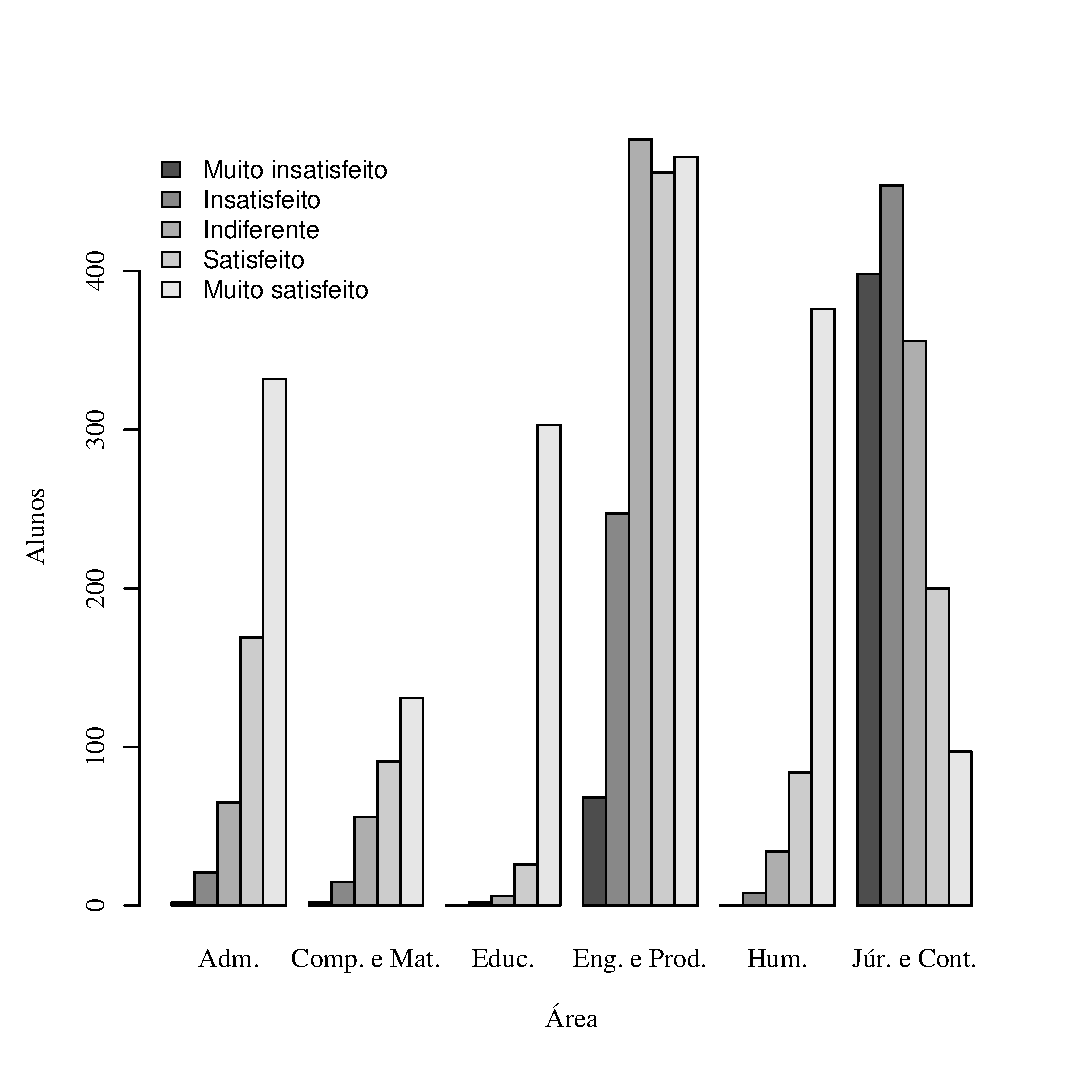
\includegraphics[scale=0.70]{plots/stacked_opiniao_por_area.eps}
	\caption{Gráfico empilhado de opinião dos alunos por área do curso.}
	\label{fig:stacked-opiniao-por-area}
\end{figure}

%\todo[inline]{Inverter eixos do gráfico da Figura \ref{fig:stacked-opiniao-por-area} para acomodar float nessa página.}
%Inverter no R não faz o float caber na página e fica estranho. Não consigo colocar a legenda fóra da área de plot e não consigo reduzir a largura (altura) das colunas.

%\FloatBarrier
\section{Pagamento por Região}
\label{section:pagamento-regiao}

As fontes de pagamento para cada uma das regiões são apresentadas em termos absolutos e percentuais na Tabela \ref{tabela: fontes de pagamento absoluto} e na Tabela \ref{tabela: fontes de pagamento percentual}, respectivamente. Adicionalmente, dados da Tabela \ref{tabela: fontes de pagamento percentual} são apresentados em formato gráfico na Figura \ref{figure: fonte de pagemento}. A composição da amostra de fonte de pagamento por região, levando em conta o número de alunos em cada região, pode ser visualizada na Figura \ref{fig:fonte de pagamento absoluto}. Para análise da variável \textit{Pagamento} agrupada por \textit{Região}, registros com valores faltantes em qualquer uma das duas variáveis foram desconsiderados.

Tanto para a região \baep quanto as demais, pode-se constar uma mudança na composição da fonte de recursos para pagamentos em relação à pesquisa anterior. Para a região \baep, a nova fonte de recursos principal é oriunda de \textit{Financiamento Bancário} (representando $53.01\%$). Em contraste com a pesquisa anterior, \textit{Incentivos Federais} agora compõem apenas $15.08\%$ dos recursos. Para as regiões \itam, \jaqu e \para, observa-se a predominância de uma única fonte de pagamento, sendo para \itam o \textit{Financiamento Bancário}, e para as demais regiões \textit{Incentivos Federais}. Por fim, para a região \arat, observa-se uma maior participação, embora não majoritária, de \textit{Incentivos Federais} na fonte de recursos (representando $47.51\%$). Cabe ressaltar que \arat e \baep apresentam composições similares para os recursos de pagamentos, porém com fontes predominantes distintas.

\begin{table}[!h]
\footnotesize
\caption{Fontes de pagamento para regiões em valores absolutos.}
\label{tabela: fontes de pagamento absoluto}
\vspace{0.5em}
\begin{tabular}{l r r r r r}
	\toprule
	\textbf{Fonte Pagamento}     & \textbf{\arat}     & \textbf{\baep}   & \textbf{\itam}  & \textbf{\jaqu} & \textbf{\para}  \\
	\midrule
	Auxílio de Familiares  & $97$       & $131$  & $10$   & $17$  & $1$    \\
	Bolsas de Estudo       & $116$      & $159$  & $7$    & $43$  & $2$    \\
	Fin. Bancário & $180$      & $1216$ & $767$  & $20$  & $0$    \\
	Incentivos Federais    & $563$      & $346$  & $3$    & $411$ & $116$  \\
	Recursos Próprios      & $226$      & $433$  & $53$   & $43$  & $1$    \\
	\bottomrule
\end{tabular}
\end{table}

\begin{table}[!h]
\footnotesize\caption{Fontes de pagamento para regiões em valores percentuais.}
\label{tabela: fontes de pagamento percentual}
\vspace{0.5em}
\begin{tabular}{l r r r r r}
	\toprule
	\textbf{Fonte Pagamento} & \textbf{\arat}     & \textbf{\baep}   & \textbf{\itam}   & \textbf{\jaqu} & \textbf{\para}  \\
	\midrule
	Auxílio de Familiares       & $8.19\%$           & $5.71\%$         & $1.19\%$         & $3.17\%$       & $0.83\%$  \\
	Bolsas de Estudo            & $9.79\%$           & $6.93\%$         & $0.83\%$         & $8.02\%$       & $1.65\%$  \\
	Fin. Bancário               & $15.19\%$          & $53.01\%$        & $90.98\%$        & $3.73\%$       & $0.0\%$   \\
	Incentivos Federais         & $47.51\%$          & $15.08\%$        & $0.36\%$         & $76.68\%$      & $95.87\%$ \\
	Recursos Próprios           & $19.07\%$          & $18.88\%$        & $6.29\%$         & $8.02\%$       & $0.83\%$  \\
	\bottomrule
\end{tabular}
\end{table}
\vspace{-3em}

\begin{figure}[h]
\begin{minipage}{0.49\textwidth}
	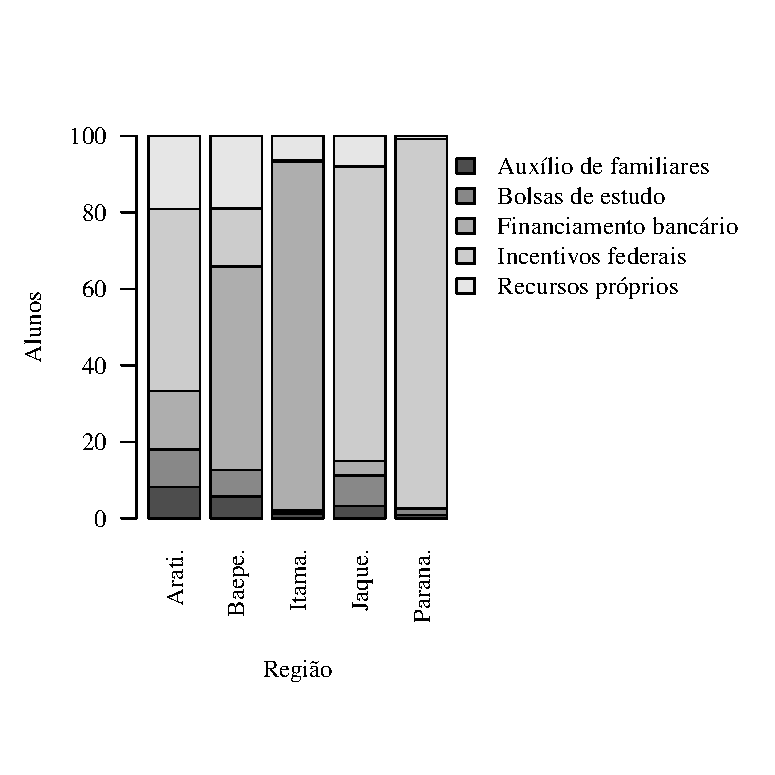
\includegraphics[width=\linewidth]{plots/stacked100_pagamento_por_regiao.eps}
	\caption{Fontes de pagamento, em percentual, por região.}
	\label{figure: fonte de pagemento}
\end{minipage}
\begin{minipage}{0.49\textwidth}
	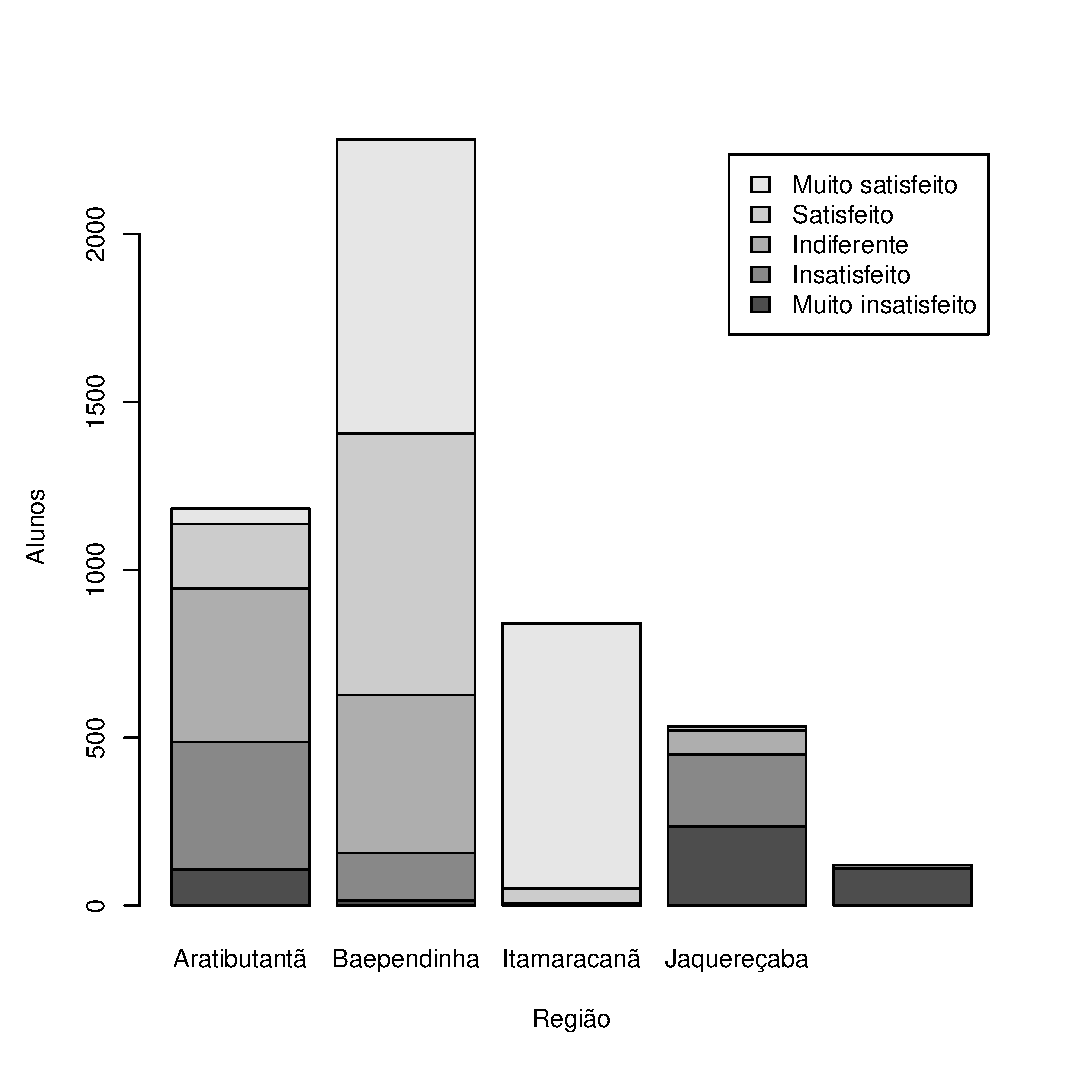
\includegraphics[width=\linewidth]{plots/stacked_pagamento_por_regiao.eps}
	\caption{Alunos por fonte de pagamento por região.}
	\label{fig:fonte de pagamento absoluto}
\end{minipage}
\end{figure}

\clearpage
\FloatBarrier
\section{Opinião por Pagamento}
\label{section:opiniao-pagamento}

A avaliação dos alunos de acordo com a fonte dos recursos para pagamento é apresentada em valores absolutos na Tabela \ref{table: avaliacao por fonte de pagamento}, e em valores relativos ao número de alunos utilizando determinada fonte na Tabela \ref{table: avaliacao por fonte de pagamento-percent}. A Figura \ref{figure: avaliacao por fonte de pagamento} mostra os mesmos dados da Tabela \ref{table: avaliacao por fonte de pagamento-percent} na forma de um gráfico de barras empilhado. Para análise da variável \textit{Opinião} agrupada por \textit{Pagamento} foram ignorados registros com valores indisponíveis em qualquer uma das variáveis. 

As fontes de recursos podem ser divididas em duas categorias: uma onde o próprio aluno paga efetivamente as mensalidades, e outra onde o o aluno não paga. O primeiro grupo é composto por \textit{Financiamento Bancário} e \textit{Recursos próprios}, enquanto o segundo é composto por \textit{Auxílio de Familiares}, \textit{Bolsas de Estudo} e \textit{Incentivos Federais}. Os resultados dessa agregação são exibidos na Tabela \ref{table:pagantes-absoluto} em valores absolutos e percentuais.

A suspeita da direção da TYU de que os alunos que recebem auxílio financeiro de alguém não são tão críticos da EAD quanto os demais não se confirma. O grupo de alunos pagantes possui avaliações significativamente melhores de seus cursos, com $83.75\%$ dos alunos avaliando os cursos como \textit{Satisfatório} ou \textit{Muito Satisfatório}. Já entre os alunos não-pagantes, apenas $18.29\%$ se declaram \textit{Satisfeitos} ou \textit{Muito Satisfeitos}, enquanto $53.26\%$ dos alunos se declararam \textit{Muito Insatisfeitos} ou \textit{Insatisfeitos} e $36.96\%$ se declaram indiferentes. Pode-se notar que os alunos não-pagantes são, na verdade, o grupo de alunos mais críticos ao EAD da TYU.

\begin{table}[h]
\footnotesize
\centering
\caption{Avaliação dos alunos pela fonte de pagamento.}
\label{table: avaliacao por fonte de pagamento}
\begin{tabular}{l rrrrrr}
\toprule
	\textbf{\specialcell{c}{Fonte Pagamento}}     & \textbf{\specialcell{c}{Muito\\insatisfeito}}    & \textbf{Insatisfeito}   & \textbf{Indiferente}  & \textbf{Satisfeito} & \textbf{\specialcell{c}{Muito\\satisfeito}} & \textbf{Total} \\
\midrule
	Auxílio de Familiares  & $4$      & $47$   & $95$   & $78$   & $33$   &\textbf{257}\\
	Bolsas de Estudo       & $22$     & $67$   & $127$  & $75$   & $37$   &\textbf{328}\\
	Fin. Bancário          & $3$      & $42$   & $192$  & $497$  & $1448$ &\textbf{2182}\\
	Incentivos Federais    & $431$    & $509$  & $354$  & $118$  & $30$   &\textbf{1442}\\
	Recursos Próprios      & $9$      & $81$   & $238$  & $260$  & $166$  &\textbf{754}\\
\midrule
	\textbf{Total} &\textbf{466} &\textbf{746}	&\textbf{1006}	&\textbf{1028}	&\textbf{1714}	&\textbf{4963}\\
\bottomrule
\end{tabular}
\end{table}

\begin{table}[h]
\footnotesize
\centering
\caption{Avaliação dos alunos pela fonte de pagamento. Valores percentuais}
\label{table: avaliacao por fonte de pagamento-percent}
\begin{tabular}{l r r r r r}
	\toprule
	\textbf{\specialcell{c}{Fonte de\\Pagamento}}     & \textbf{\specialcell{c}{Muito\\insatisfeito}}     & \textbf{Insatisfeito}   & \textbf{Indiferente}  & \textbf{Satisfeito} & \textbf{\specialcell{c}{Muito\\satisfeito}}  \\
\midrule
	Auxílio de Familiares  & $1.56\%$    & $18.29\%$    & $36.96\%$   & $30.35\%$  & $12.84\%$  \\
	Bolsas de Estudo       & $6.71\%$    & $20.43\%$    & $38.72\%$   & $22.87\%$  & $11.28\%$  \\
	Financiamento Bancário & $0.14\%$    & $1.92\%$     & $8.80\%$    & $22.78\%$  & $66.36\%$  \\
	Incentivos Federais    & $29.89\%$   & $35.30\%$    & $24.55\%$   & $8.18\%$   & $2.08\%$   \\
	Recursos Próprios      & $1.19\%$    & $10.74\%$    & $31.56\%$   & $34.48\%$  & $22.02\%$  \\
\bottomrule
\end{tabular}
\end{table}
%           Mins ins   indif sats  Msats   Total
% Paga      12   123   430   757   1614    2936
% Não paga  457  623   576   271   100     2027

\begin{figure}[h]
\centering
\begin{minipage}{\textwidth}
\footnotesize
\centering
\captionof{table}{Números de avaliações para alunos nas categorias agrupadas de pagantes e não-pagantes.}
\label{table:pagantes-absoluto}
\begin{tabular}{l c c c c c c}
	\toprule
	\textbf{Categoria}     & \textbf{\specialcell{c}{Muito\\insatisfeito}}     & \textbf{Insatisfeito}   & \textbf{Indiferente}  & \textbf{Satisfeito} & \textbf{\specialcell{c}{Muito\\satisfeito}} & \textbf{Total} \\
	\midrule
	%              & M Insatisf.     & Insatisf.       & Indif.          & Satisf.         & M Satisf.        & Total
	Pagante        & 12   & 123  & 430  & 757  & 1614  & \textbf{2936} \\
	Não-pagante    & 457  & 623  & 576  & 271  & 100   & \textbf{2027} \\
	\midrule
	\textbf{Total} & \textbf{469}             & \textbf{746}             & \textbf{1006}            & \textbf{10028}           & \textbf{1714}             & \textbf{4963} \\
	\bottomrule
\end{tabular}
\end{minipage}
\\
\vspace{3em}
\begin{minipage}{\textwidth}
\footnotesize
\centering
\captionof{table}{Avaliações para alunos pagantes e não-pagantes. Valores percentuais.}
\label{table:pagantes-percentual}
\begin{tabular}{l c c c c c c}
	\toprule
	\textbf{Categoria}     & \textbf{\specialcell{c}{Muito\\insatisfeito}}     & \textbf{Insatisfeito}   & \textbf{Indiferente}  & \textbf{Satisfeito} & \textbf{\specialcell{c}{Muito\\satisfeito}} \\
	\midrule
	%              & M Insatisf.     & Insatisf.       & Indif.          & Satisf.         & M Satisf.        & Total
	Pagante        & $0.40\%$   & $4.18\%$  & $36.96\%$ & $25.78\%$ & $57.97\%$ \\
	Não-pagante    & $22.54\%$  & $30.73\%$ & $36.96\%$ & $13.36\%$ & $4.93\%$ \\
	\bottomrule
\end{tabular}
\end{minipage}
\end{figure}

\begin{figure}[h]
\begin{minipage}{0.49\textwidth}
	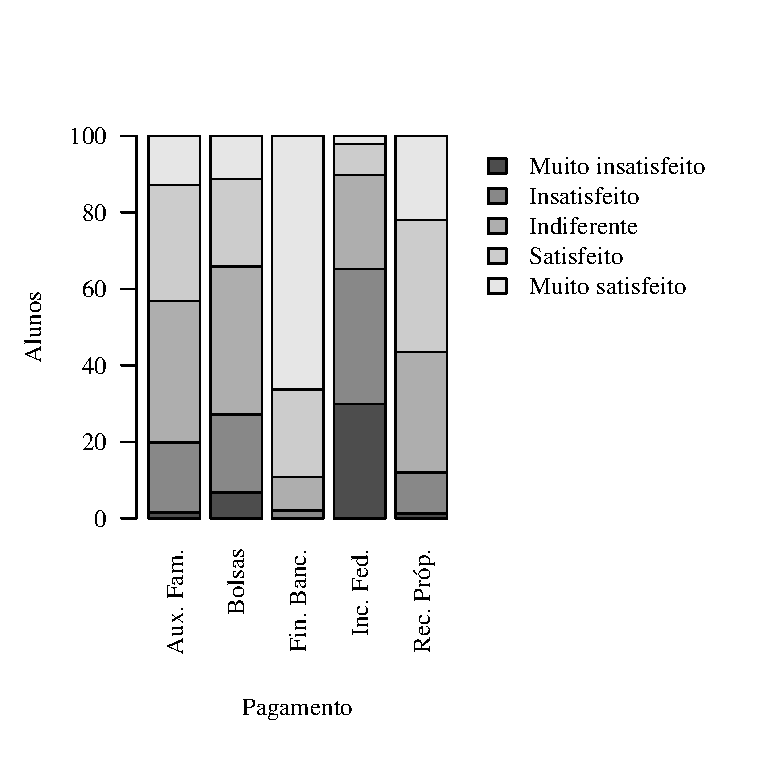
\includegraphics[width=\linewidth]{plots/stacked_opiniao_por_pagamento.eps}
	\caption{Avaliação dos alunos pela fonte de pagamento}
	\label{figure: avaliacao por fonte de pagamento}
\end{minipage}
%
\begin{minipage}{0.49\textwidth}
	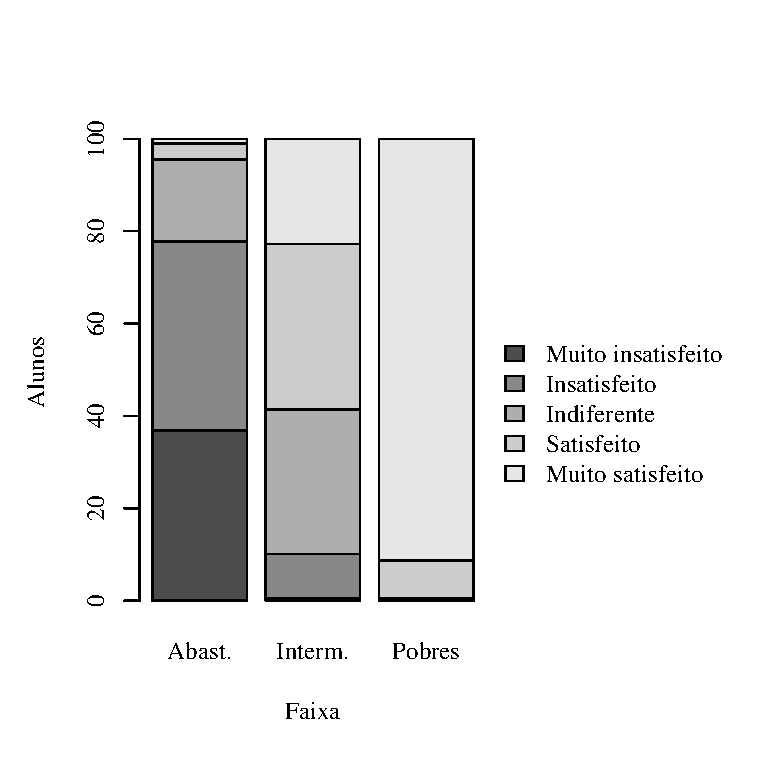
\includegraphics[width=\linewidth]{plots/stacked_opiniao_por_faixaRenda.eps}
	\caption{Satisfação dos alunos de acordo com classes de renda.}
	\label{fig:satisfacao-renda}
\end{minipage}
\end{figure}


%           Mins  ins   indif  sats   Msats   Total
% Paga      0.40  4.18  14.64  25.78  54.97    2936
% Não paga  22.54 30.73 28.41  13.36  4.93     2027

\FloatBarrier

\section{Opinião por Renda}
\label{section:opiniao-renda}

Para dividir a amostra em conjuntos de alunos pobres, alunos com renda intermediária e alunos abastados foram utilizados os valores dos quartis inferior e superior. O quartil inferior foi calculado em $1.35$ salários mínimos, o que foi usado para definir todos os alunos com renda menor ou igual a $1.35$ salários como pobres. Similarmente, todos os alunos com renda maior ou igual ao quartil superior ($2.73$ salários mínimos) foram considerados como abastados. Os alunos com renda maior que $1.35$ e menor que $2.73$ foram considerados como de renda intermediária. Usando essa divisão de classes, a contagem e percentuais associados exibidos na Tabela \ref{fig:satisfacao-renda} foram obtidos. A Figura \ref{fig:satisfacao-renda} mostra um gráfico empilhado com a distribuição das avaliações de acordo com a classe de renda. Para esta análise, registros com valores faltantes nas variáveis \textit{Opinião} ou \textit{Renda} foram desconsiderados.

% Ab -> indif || Ab -> insatisf
% pobre -> satisf || pobre -> satisf
% int -> insatif. || int -> satisf

Observando as proporções na Tabela \ref{table:satisfaca-renda}, pode ser percebida uma mudança em relação às conclusões da pesquisa anterior. Os alunos mais abastados, então indiferentes, hoje estão $77.73\%$ insatisfeitos ou muito insatisfeitos com seus cursos, sendo que apenas $4.49\%$ se declararam satisfeitos ou muito satisfeitos. Outra mudança após os 10 anos é que alunos com renda classificada como intermediária passaram de majoritariamente indiferentes, para majoritariamente ($58.57\%$) satisfeitos ou muito satisfeitos. A única classe de alunos que não sofreu mudança foi a dos alunos pobres, dos quais $91.34\%$ estão muito satisfeitos, e $8.18\%$ estão satisfeitos. Somando alunos pobres satisfeitos ou muito satisfeitos, obtém-se $99.52\%$ dos alunos pobres.

\begin{table}[h]
\centering
\footnotesize
\caption{Satisfação de alunos de acordo com classes de renda. Valores percentuais}
\label{table:satisfacao-percentual-renda}
\begin{tabular}{l r r r r r r}
\toprule
\textbf{Classe} & \textbf{\specialcell{c}{Muito\\insatisfeito}}     & \textbf{Insatisfeito}   & \textbf{Indiferente}  & \textbf{Satisfeito} & \textbf{\specialcell{c}{Muito\\satisfeito}}  \\
\midrule
%                & M Insatsf.      & Insats.         & Indif.          & Satisf.         & Muito Satisf.    & Total         \\ 
	Pobres         & $0\%$     & $0\%$     & $0.48\%$  & $8.18\%$  & $91.34\%$ \\
	Intermediário  & $0.49\%$  & $9.63\%$  & $31.31\%$ & $35.84\%$ & $22.73\%$ \\
 	Abastados      & $36.86\%$ & $40.87\%$ & $17.79\%$ & $3.53\%$  & $0.96\%$  \\
\bottomrule
\end{tabular}
\end{table}

\begin{table}[h]
\centering
\footnotesize
\caption{Satisfação alunos de acordo com classes de renda.}
\label{table:satisfaca-renda}
\begin{tabular}{l r r r r r r}
\toprule
\textbf{Classe} & \textbf{\specialcell{c}{Muito\\insatisfeito}}     & \textbf{Insatisfeito}   & \textbf{Indiferente}  & \textbf{Satisfeito} & \textbf{\specialcell{c}{Muito\\satisfeito}} & \textbf{Total}  \\
\midrule
%                  & M Insatsf.         & Insats.         & Indif.          & Satisf.         & Muito Satisf.    & Total         \\ 
	Pobres         & 0        & 0       & 6        & 102  & 1139 & \textbf{1247} \\
	Intermediário  & 12       & 238     & 774      & 886  & 562  & \textbf{2472} \\
 	Abastados      & 460      & 510     & 222      & 44   & 12   & \textbf{1248} \\
\midrule
  \textbf{Total} & \textbf{472}    & \textbf{748}    & \textbf{1002}   & \textbf{1032}   & \textbf{1713}    & \textbf{4967} \\
\bottomrule
\end{tabular}
\end{table}

\FloatBarrier
\section{Opinião por Idade}
\label{section:opiniao-idade}

A correlação entre alunos mais velhos com o grau de satisfação em seus cursos é apresentada na Tabela \ref{tabela: correlacao idade cursos absoluta} e na Tabela \ref{tabela: correlacao idade cursos percentual} em termos absolutos e percentuais, respectivamente. Além disso, a Figura \ref{fig:stacked-opiniao-por-idade} sintetiza de forma gráfica os valores apresentados na Tabela  \ref{tabela: correlacao idade cursos absoluta}.

Em contraste com 10 anos atrás, quando o EAD iniciou suas atividades, percebe-se que no estudo atual houve uma inversão da avaliação dos alunos velhos e jovens quanto ao  seus cursos. A maioria dos alunos jovens estão satisfeitos ou muito satisfeitos com o curso ($90.73\%$). Os alunos mais velhos apresentam uma distribuição de opiniões mais uniforme onde a opinião mais popular é a indiferença com $25.62\%$ dos alunos. Há mais alunos velhos com opiniões positivas ($39.56\%$) do que alunos com opiniões negativas ($36.82\%$), então pode-se afirmar que os alunos mais velhos ainda estão mais satisfeitos ou indiferentes com relação ao seu curso. No entanto, diferentemente do passado, os alunos jovens estão muito mais satisfeitos que os alunos mais velhos.

\begin{table}[!h]
\footnotesize
\centering
\caption{Correlação absoluta de alunos novos e velhos com grau de satisfação com seus cursos.}
\vspace{0.5em}
\label{tabela: correlacao idade cursos absoluta}
\begin{tabular}{l r r r r r r}
	\toprule
	\textbf{Alunos}	& \textbf{\specialcell{c}{Muito\\Insatisfeito}} & \textbf{Insatisfeito} & \textbf{Indiferente} & \textbf{Satisfeito} & \textbf{\specialcell{c}{Muito\\Satisfeito}} & \textbf{Total} \\
	\midrule
	%                                M Ins  & Ins    & Indif  & Satisf  & M Satisf & Total
	\specialcell{c}{Alunos Jovens\\($< 30$ anos)}     & $5$    & $15$   & $122$  & $278$   & $1111$   & $1531$  \\
	\specialcell{c}{Alunos Velhos\\($\geq 30$ anos)} & $467$  & $734$  & $467$  & $608$   & $757$    & $3450$  \\
	\midrule{}
	\textbf{Total}                 & $472$  & $749$  & $1006$ & $1035$  & $1719$   & $4981$  \\
	\bottomrule
\end{tabular}
\end{table}

\begin{table}[!h]
\footnotesize
\centering
\caption{Correlação percentual de alunos novos e velhos com grau de satisfação com seus cursos.}
\vspace{0.5em}
\label{tabela: correlacao idade cursos percentual}
\begin{tabular}{l r r r r r}
	\toprule
	\textbf{Alunos}                & \textbf{\specialcell{c}{Muito\\Insatisfeito}} & \textbf{Insatisfeito} & \textbf{Indiferente} & \textbf{Satisfeito} & \textbf{\specialcell{c}{Muito\\Satisfeito}} \\
	\midrule
	%                              & M Insatisf  & Insatisf   & Indif      &	 Satisf      &  M Satisf  \\
	Alunos Jovens ($< 30$ anos)     & $0.33\%$    & $0.98\%$   & $7.97\%$  & $18.16\%$   & $72.57\%$  \\
	Alunos Velhos ($\geq 30$ anos) & $15.54\%$   & $21.28\%$  & $25.62\%$  & $21.94\%$  & $17.62\%$  \\
	\bottomrule
\end{tabular}
\end{table}

\begin{figure}[!h]
	\centering
	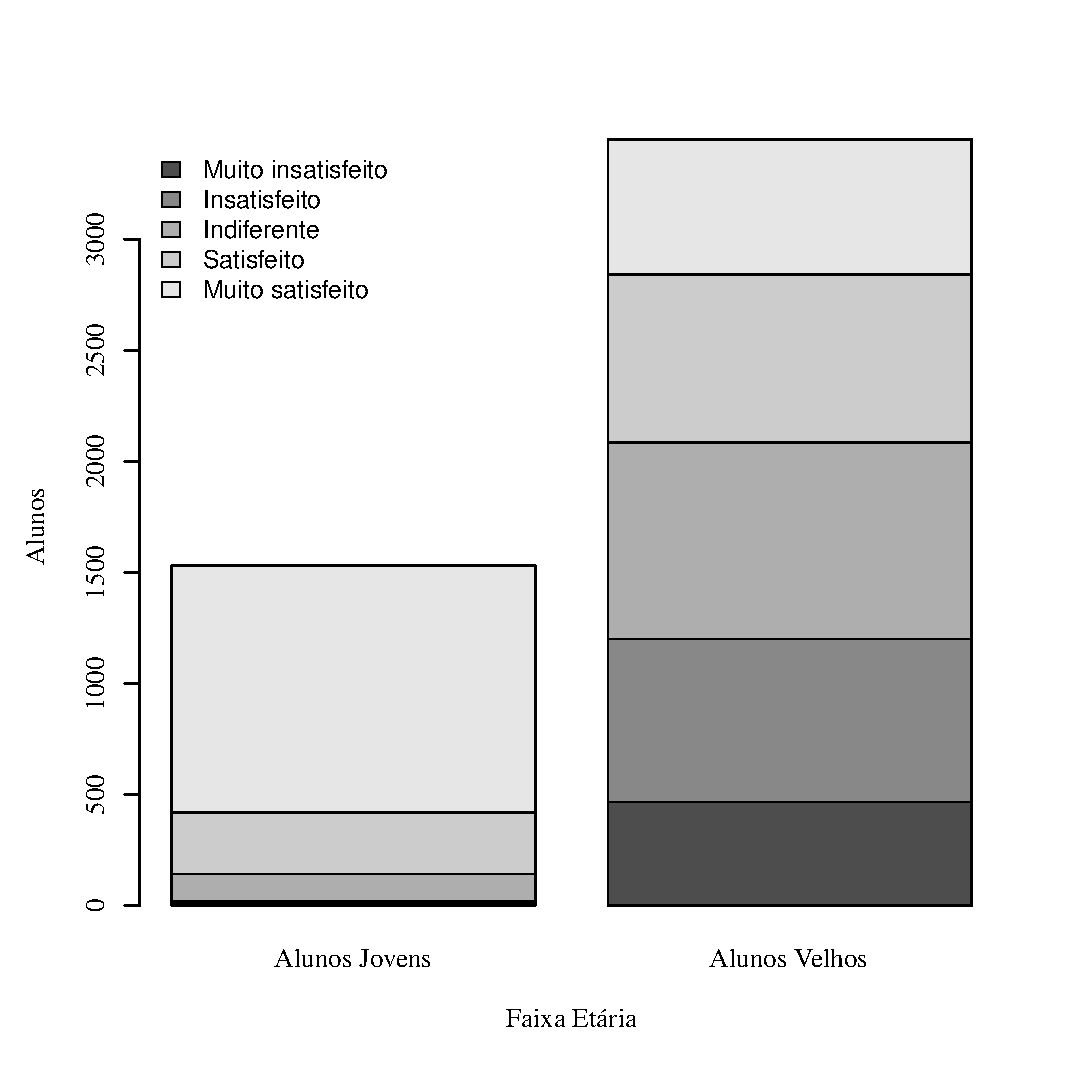
\includegraphics[width=.6\linewidth]{plots/stacked_opiniao_por_idade.eps}
	\caption{Gráfico empilhado de \textit{Opinião} por \textit{Faixa Etária}}
	\label{fig:stacked-opiniao-por-idade}
\end{figure}

\FloatBarrier
\clearpage
\begin{center}
\section*{Parte 4: Análise em Conjunto de Mais de Duas Variáveis}
\end{center}

\section{Opinião por Região e Área}
\label{section:opiniao-regiao-area}

A Tabela \ref{tabela:q15p} apresenta a proporção de alunos para cada nível de satisfação, agrupados por Região e Área do curso, e a tabela \ref{tabela:q15a} apresenta os mesmos dados em valores absolutos. Em contraste, a Tabela \ref{table:opiniao-por-area} da Seção \ref{section:opiniao-area} apresenta essas proporções apenas por área, ignorando a região. Novamente, na construção da Tabelas \ref{tabela:q15a} e \ref{tabela:q15p} foram desconsiderados registros com valores perdidos em quaisquer uma das três variáveis (\textit{Região}, \textit{Área} e \textit{Opinião}) envolvidas. 

% latex table generated in R 3.2.4 by xtable 1.8-2 package
% Fri Apr  8 20:51:25 2016
\begin{table}[ht]
\centering
\begin{tabular}{ll rrrrr}
  \toprule
 Área                    & Região $\vert$ Opinião & \multicolumn{1}{l}{ Muito insatisfeito} & \multicolumn{1}{l}{ Insatisfeito} & \multicolumn{1}{l}{ Indiferente} & \multicolumn{1}{l}{ Satisfeito} & \multicolumn{1}{l}{ Muito satisfeito} \\ 
   \midrule
Administração           & Aratibutantã            &                  0 &           12 &          23 &         32 &                8 \\ 
                          & Baependinha             &                  1 &            8 &          38 &        121 &              171 \\ 
                          & Itamaracanã             &                  0 &            0 &           0 &         11 &              152 \\ 
                          & Jaquereçaba             &                  1 &            1 &           4 &          2 &                0 \\ 
                          & Paranapitanga           &                  0 &            0 &           0 &          0 &                0 \\ 
\midrule
 Computação e Matemática & Aratibutantã            &                  1 &            8 &          25 &         20 &                6 \\ 
                          & Baependinha             &                  0 &            5 &          26 &         63 &               83 \\ 
                          & Itamaracanã             &                  0 &            0 &           2 &          7 &               41 \\ 
                          & Jaquereçaba             &                  1 &            2 &           3 &          1 &                0 \\ 
                          & Paranapitanga           &                  0 &            0 &           0 &          0 &                0 \\ 
\midrule
 Educacional             & Aratibutantã            &                  0 &            1 &           1 &          4 &                1 \\ 
                          & Baependinha             &                  0 &            1 &           5 &         22 &               87 \\ 
                          & Itamaracanã             &                  0 &            0 &           0 &          0 &              212 \\ 
                          & Jaquereçaba             &                  0 &            0 &           0 &          0 &                0 \\ 
                          & Paranapitanga           &                  0 &            0 &           0 &          0 &                0 \\ 
\midrule
  Engenharia e Produção   & Aratibutantã            &                 20 &          133 &         220 &         77 &               22 \\ 
                          & Baependinha             &                  5 &           44 &         224 &        356 &              300 \\ 
                          & Itamaracanã             &                  0 &            0 &           4 &         19 &              149 \\ 
                          & Jaquereçaba             &                 32 &           69 &          34 &          6 &                0 \\ 
                          & Paranapitanga           &                 10 &            1 &           0 &          0 &                0 \\ 
\midrule
  Humanidades             & Aratibutantã            &                  0 &            3 &          10 &         14 &                5 \\ 
                          & Baependinha             &                  0 &            3 &          23 &         65 &              163 \\ 
                          & Itamaracanã             &                  0 &            0 &           0 &          4 &              207 \\ 
                          & Jaquereçaba             &                  0 &            1 &           1 &          1 &                0 \\ 
                          & Paranapitanga           &                  0 &            0 &           0 &          0 &                0 \\ 
\midrule
  Jurídica e Contábil     & Aratibutantã            &                 86 &          222 &         173 &         44 &                2 \\ 
                          & Baependinha             &                  9 &           81 &         152 &        151 &               68 \\ 
                          & Itamaracanã             &                  0 &            0 &           1 &          3 &               26 \\ 
                          & Jaquereçaba             &                200 &          141 &          30 &          2 &                0 \\ 
                          & Paranapitanga           &                101 &            9 &           0 &          0 &                0 \\ 
   \bottomrule
\end{tabular}
\end{table}


% latex table generated in R 3.2.4 by xtable 1.8-2 package
% Mon Apr 11 13:06:19 2016
\begin{table}[ht]
\scriptsize
\centering
\caption{Opinião por Área e por Região em valores percentuais} 
\vspace{.5em}
\label{tabela:q15p}
\begin{tabular}{ll rrrrr}
  \toprule
 \textbf{Área} & \textbf{Região}  & \textbf{\specialcell{c}{Muito\\Insatisfeito}} & \textbf{ Insatisfeito} & \textbf{ Indiferente} & \textbf{ Satisfeito} & \textbf{\specialcell{c}{Muito\\Satisfeito}} \\ 
   \midrule
Administração             & Aratibutantã            &               0.00 &        16.00 &       30.67 &      42.67 &            10.67 \\ 
                          & Baependinha             &               0.29 &         2.36 &       11.21 &      35.69 &            50.44 \\ 
                          & Itamaracanã             &               0.00 &         0.00 &        0.00 &       6.75 &            93.25 \\ 
                          & Jaquereçaba             &              12.50 &        12.50 &       50.00 &      25.00 &             0.00 \\ 
                          & Paranapitanga           &               0.00 &         0.00 &        0.00 &       0.00 &             0.00 \\ 
 \midrule{}
						  & Aratibutantã            &               1.67 &        13.33 &       41.67 &      33.33 &            10.00 \\ 
                          & Baependinha             &               0.00 &         2.82 &       14.69 &      35.59 &            46.89 \\ 
  Computação e            & Itamaracanã             &               0.00 &         0.00 &        4.00 &      14.00 &            82.00 \\ 
  Matemática          	  & Jaquereçaba             &              14.29 &        28.57 &       42.86 &      14.29 &             0.00 \\ 
                          & Paranapitanga           &               0.00 &         0.00 &        0.00 &       0.00 &             0.00 \\ 
 \midrule{}
						  & Aratibutantã            &               0.00 &        14.29 &       14.29 &      57.14 &            14.29 \\ 
                          & Baependinha             &               0.00 &         0.87 &        4.35 &      19.13 &            75.65 \\ 
   Educacional            & Itamaracanã             &               0.00 &         0.00 &        0.00 &       0.00 &           100.00 \\ 
                          & Jaquereçaba             &               0.00 &         0.00 &        0.00 &       0.00 &             0.00 \\ 
                          & Paranapitanga           &               0.00 &         0.00 &        0.00 &       0.00 &             0.00 \\ 
 \midrule{}
						  & Aratibutantã            &               4.24 &        28.18 &       46.61 &      16.31 &             4.66 \\ 
                          & Baependinha             &               0.54 &         4.74 &       24.11 &      38.32 &            32.29 \\ 
  Engenharia e            & Itamaracanã             &               0.00 &         0.00 &        2.33 &      11.05 &            86.63 \\ 
  Produção                & Jaquereçaba             &              22.70 &        48.94 &       24.11 &       4.26 &             0.00 \\ 
                          & Paranapitanga           &              90.91 &         9.09 &        0.00 &       0.00 &             0.00 \\ 
 \midrule{}
						  & Aratibutantã            &               0.00 &         9.38 &       31.25 &      43.75 &            15.62 \\ 
                          & Baependinha             &               0.00 &         1.18 &        9.06 &      25.59 &            64.17 \\ 
  Humanidades             & Itamaracanã             &               0.00 &         0.00 &        0.00 &       1.90 &            98.10 \\ 
                          & Jaquereçaba             &               0.00 &        33.33 &       33.33 &      33.33 &             0.00 \\ 
                          & Paranapitanga           &               0.00 &         0.00 &        0.00 &       0.00 &             0.00 \\ 
 \midrule{}
						  & Aratibutantã            &              16.32 &        42.13 &       32.83 &       8.35 &             0.38 \\ 
    Jurídica e         	  & Baependinha             &               1.95 &        17.57 &       32.97 &      32.75 &            14.75 \\ 
	Contábil			  & Itamaracanã             &               0.00 &         0.00 &        3.33 &      10.00 &            86.67 \\ 
						  & Jaquereçaba             &              53.62 &        37.80 &        8.04 &       0.54 &             0.00 \\ 
                          & Paranapitanga           &              91.82 &         8.18 &        0.00 &       0.00 &             0.00 \\ 
   \bottomrule
\end{tabular}
\label{tabela:q15p}
\end{table}



Os cursos da área \edu, quando avaliados em toda a TYU apresentaram melhora, com $89.91\%$ dos alunos muito satisfeitos. Analisando cada região separadamente, \arat possui apenas 7 alunos, dos quais a maioria estão apenas satisfeitos ($57.14\%$), o que é um valor acima da média de alunos satisfeitos para todas as regiões ($7.72$), porém apenas $14.29\%$ dos alunos estão muito satisfeitos, o que é um valor abaixo da média. \baep, possui um número razoável de alunos, totalizando 115, dos quais $19.14\%$ estão satisfeitos (acima da média) e $75.65\%$ estão muito satisfeitos (abaixo da média), porém é um valor que apresenta melhoria significativa em comparação à última pesquisa. Já em \itam todos os 212 alunos da área \edu, que constituem $67.52\%$ dos alunos da área educacional para todas as regiões, estão muito satisfeitos. As regiões de \jaqu e \para não possuem alunos da área \edu. Conclui-se que de fato todos os polos apresentaram melhoria na opinião dos alunos, mas \arat e \baep apresentam índices inferiores ao maior polo em \itam.

Os cursos da área \hum apresentaram um total de $74.9\%$ de alunos muito satisfeitos, mas observando-se as Tabelas \ref{tabela:q15p} e \ref{tabela:q15a}, novamente observa-se que em \itam, que contem $42.2\%$ do total de alunos, possui  $98.10\%$ de alunos muito satisfeitos, enquanto em \arat e \baep apenas $15.62\%$ e $64.17\%$ dos alunos, respectivamente, possuem a mesma opinião. Mesmo assim, tanto \arat quanto \baep possuem, majoritariamente alunos satisfeitos ou muito satisfeitos contabilizando, respectivamente, $59.37\%$ e $89.76\%$. Já \jaqu possui apenas 3 alunos, sendo 1 insatisfeito, 1 indiferente e 1 satisfeito, sendo uma opinião insignificante perante a quantidade total de alunos de todas as regiões. A cidade de \para não possui alunos da área \hum. Nota-se, portanto, que as observações da questão da Seção \ref{section:opiniao-area} ainda se mantém, pois não há alunos muito insatisfeitos.

Para a área \comp, temos que $44.41\%$ do total de alunos estão muito satisfeitos e $30.85\%$ estão satisfeitos, totalizando $75.26\%$ com algum grau de satisfação.
De acordo com a tabela \ref{tabela:q15p}, a cidade de \arat , que possui 60 alunos, apresenta $33.33\%$ de alunos satisfeitos e apenas $10\%$ de alunos muitos satisfeitos, o que é um valor abaixo da média, e $41.67\%$dos alunos são indiferentes, um valor acima da média. Em contrapartida, nas cidades de \baep e \itam observa-se que $80.48\%$ e $96\%$ dos seus alunos, respectivamente, estão satisfeitos ou muito satisfeitos com o seu curso, valores condizentes com a média observada na Seção \ref{section:opiniao-area}. Por outro lado, na cidade de \jaqu $42.86\%$ dos alunos estão insatisfeitos ou muito insatisfeitos e apenas $14.29\%$ estão satisfeitos e não apresenta alunos muito satisfeitos, o que não condiz com a média observada. Conclui-se que para a area \comp as cidades de \baep e \itam apresentam resultados conforme a pesquisa anterior, na cidade de \arat a quantidade de alunos que apresenta grau de satisfação e indiferença são próximos e os alunos da cidade de \jaqu estão insatisfeitos com o seu curso.

Para a área \adm, temos que $56.37\%$ do total de alunos estão muito satisfeitos e $28.69\%$ estão satisfeitos, totalizando $85.06\%$ de alunos com algum grau de satisfação. Nas cidades de \baep e \itam $86.13\%$ e $100\%$ dos seus alunos, respectivamente, apresentam grau de satisfação. Entretanto, na cidade de \arat $53.34\%$ do total de alunos apresentam grau de satisfação e $30.67\%$ são indiferentes, enquanto que na cidade de \jaqu $25\%$ dos alunos apresentam grau de insatisfação, $50\%$ são indiferentes e apenas $25\%$ estão satisfeitos. Ou seja, apenas as cidades de \baep e \itam apresentam resultados de acordo com a pesquisa anterior. 

Na área de \eng, temos que $53.92\%$ do total de alunos apresentam algum grau de satisfação. Para as cidades de \baep e \itam $70.61\%$ e $97.67\%$, respectivamente, apresentam grau de satisfação, porém na cidade de \arat os alunos são predominantemente indiferentes ($46.61\%$) e nas cidades de \jaqu e \para os alunos predominantemente apresentam grau de insatisfação ($71.64\%$ $100\%$, respectivamente). Conclui-se que os investimentos que foram realizados nos cursos da área \eng a fim de aumentar a satisfação dos seus alunos deram resultados somente nas cidades de \baep e \itam.{}

Na área \jur, temos que $56.62\%$ do total de alunos apresentam um grau de insatisfação e apenas $19.74\%$ estão satisfeitos. De acordo com a tabela{\ref:tabela:q15p} observa-se que a insatisfação dos alunos é predominante nas cidades de \arat, \jaqu e \para ($58.45\%$,  $91.42\%$ e $100\%$, respectivamente), por outro lado nas cidades de \baep e \itam existe uma predominancia de satisfação ($47.5\%$ em um total de 461 alunos e $96.67\%$ em um total de 30 alunos, respectivamente). Pode-se concluir que, de acordo com a Seção \ref{section:opiniao-area}, os investimentos para a área \jur deram resultados apenas para as cidades de \baep e \itam, mas não foram o suficiente nas demais regiões.

No geral, podemos concluir que os investimentos realizados pela TYU para aumentar a satisfação dos seus alunos em seus cursos surtiram um maior efeito nas regiões de \arat, \baep e \itam. Para os cursos das regiões \jaqu e \para é necessário realizar um maior investimento ou abordar uma nova estratégia para aumentar a satisfação de seus alunos.

\FloatBarrier
\section{Opinião por Renda e Área}
\label{section:opiniao-renda-area}

A Tabela \ref{tabela:q16p} apresenta a proporção de alunos para cada nível de satisfação, agrupados por Classe de Renda e Região do curso, e a tabela \ref{tabela:q16} apresentam estes dados em valores absolutos. Em contraste, a Tabela \ref{table:satisfaca-renda} da Seção \ref{section:opiniao-renda} apresenta essas proporções apenas por classe de renda, ignorando a região. Os resultados apresentados na Seção \ref{section:opiniao-renda} indicam que os alunos mais abastados estão insatisfeitos com seus cursos, os de renda intermediária são indiferentes e que os mais pobres são mais satisfeitos com seu curso. Ressaltamos que na construção das Tabelas \ref{tabela:q16} e \ref{tabela:q16p} foram desconsiderados registros com valores perdidos em quaisquer uma das três variáveis (\textit{Renda}, \textit{Área} e \textit{Opinião}) envolvidas. 

% latex table generated in R 3.2.4 by xtable 1.8-2 package
% Fri Apr  8 21:31:49 2016
\begin{table}[ht]
\centering
\begin{tabular}{ll rrrrr}
  \toprule
 Classe        & Região $\vert$ Opinião & \multicolumn{1}{l}{ Muito insatisfeito} & \multicolumn{1}{l}{ Insatisfeito} & \multicolumn{1}{l}{ Indiferente} & \multicolumn{1}{l}{ Satisfeito} & \multicolumn{1}{l}{ Muito satisfeito} \\ 
   \midrule
Abastados     & Aratibutantã            &                101 &          263 &         127 &         16 &                1 \\ 
                & Baependinha             &                 11 &           58 &          54 &         25 &                7 \\ 
                & Itamaracanã             &                  0 &            0 &           0 &          0 &                4 \\ 
                & Jaquereçaba             &                234 &          178 &          41 &          3 &                0 \\ 
                & Paranapitanga           &                111 &           10 &           0 &          0 &                0 \\ 
  Intermediario & Aratibutantã            &                  6 &          118 &         329 &        173 &               40 \\ 
                & Baependinha             &                  4 &           84 &         411 &        670 &              450 \\ 
                & Itamaracanã             &                  0 &            0 &           6 &         30 &               76 \\ 
                & Jaquereçaba             &                  2 &           36 &          31 &          9 &                0 \\ 
                & Paranapitanga           &                  0 &            0 &           0 &          0 &                0 \\ 
  Pobres        & Aratibutantã            &                  0 &            0 &           0 &          4 &                4 \\ 
                & Baependinha             &                  0 &            0 &           5 &         84 &              419 \\ 
                & Itamaracanã             &                  0 &            0 &           1 &         14 &              710 \\ 
                & Jaquereçaba             &                  0 &            0 &           0 &          0 &                0 \\ 
                & Paranapitanga           &                  0 &            0 &           0 &          0 &                0 \\ 
   \bottomrule
\end{tabular}
\end{table}


% latex table generated in R 3.2.4 by xtable 1.8-2 package
% Mon Apr 11 17:35:47 2016
\begin{table}[h]
\scriptsize
\centering
\caption{Grau de satisfação dos alunos por classe econômica e região em valores percentuais}
\label{tabela:q16p}
\vspace{0.5em}
\begin{tabular}{ll rrrrr}
\toprule
\textbf{\specialcell{c}{Classe de \\Renda}}   & \textbf{Região}  & \textbf{\specialcell{c}{Muito\\insatisfeito}} & \textbf{Insatisfeito} & \textbf{Indiferente} & \textbf{Satisfeito} & \textbf{\specialcell{c}{Muito\\satisfeito}}\\
\midrule
Abastados     & Aratibutantã              &              19.88\% &        51.77\% &       25.00\% &       3.15\% &             0.20\% \\ 
                & Baependinha             &               7.10\% &        37.42\% &       34.84\% &      16.13\% &             4.52\% \\ 
                & Itamaracanã             &               0.00\% &         0.00\% &        0.00\% &       0.00\% &           100.00\% \\ 
                & Jaquereçaba             &              51.32\% &        39.04\% &        8.99\% &       0.66\% &             0.00\% \\ 
                & Paranapitanga           &              91.74\% &         8.26\% &        0.00\% &       0.00\% &             0.00\% \\ 
\midrule                                                                                                                           
     Intermediario & Aratibutantã         &               0.90\% &        17.77\% &       49.40\% &      25.90\% &             6.02\% \\ 
                & Baependinha             &               0.25\% &         5.22\% &       25.34\% &      41.49\% &            27.70\% \\ 
                & Itamaracanã             &               0.00\% &         0.00\% &        5.45\% &      27.27\% &            67.27\% \\ 
                & Jaquereçaba             &               2.60\% &        45.45\% &       40.26\% &      11.69\% &             0.00\% \\ 
                & Paranapitanga           &               0.00\% &         0.00\% &        0.00\% &       0.00\% &             0.00\% \\ 
\midrule                                                                                                                           
     Pobres        & Aratibutantã         &               0.00\% &         0.00\% &        0.00\% &      50.00\% &            50.00\% \\ 
                & Baependinha             &               0.00\% &         0.00\% &        0.98\% &      16.54\% &            82.48\% \\ 
                & Itamaracanã             &               0.00\% &         0.00\% &        0.14\% &       1.93\% &            97.93\% \\ 
                & Jaquereçaba             &               0.00\% &         0.00\% &        0.00\% &       0.00\% &             0.00\% \\ 
                & Paranapitanga           &               0.00\% &         0.00\% &        0.00\% &       0.00\% &             0.00\% \\ 
\bottomrule
\end{tabular}
\end{table}



De acordo com as tabelas \ref{tabela:q16} e \ref{tabela:q16p}, dos alunos que são mais abastados, os que pertencem as regiões \arat, \baep, \jaqu e \para apresentam um alto grau de insatisfação, correspondendo à $71.65\%$, $44.52\%$, $90.36\%$ e $100\%$, respectivamente. Apenas os alunos da região \itam estão muito satisfeitos, porém eles correspondem à apenas $0.32\%$ da quantidade total de alunos abastados.

Para os alunos de renda intermediária, os que estudam na cidades de \arat são em sua maioria indiferentes ($49.4\%$), os alunos de \baep e \itam apresentam um maior grau de satisfação ($69.6\%$ e $94.54\%$, respectivamente) e os alunos de \jaqu são em sua maioria insatisfeitos~($48.05\%$).

Para os alunos pobres, observa-se que eles são, praticamente, satisfeitos ou muitos satisfeitos com os seus cursos. Nas cidades de \baep e \itam menos de $1\%$ de todos os alunos pobres são indiferentes. Portanto, pode-se concluir que, assim como indicado na Seção \ref{section:opiniao-renda}, os alunos mais pobres são satisfeitos ou muitos satisfeitos com seus cursos, independente da sua região. 

\FloatBarrier
\clearpage
\begin{center}
\section*{Parte 5: Recomendações para o Cliente}
\end{center}

\section{Recomendação para o Cliente: Estimativa}
\label{section:estimativa}

Para avaliar a opinião dos alunos de EAD da TYU de acordo com as variáveis \textit{Região}, \textit{Idade} e \textit{Pagamento}, pode-se construir uma tabela de frequência das opiniões relacionados aos valores filtrados das variáveis em questão. Para apresentação visual, gráficos de setores para cada conjunto de alunos são mais adequados. Conforme detalhado a seguir, em comparação com os dados da Tabela \ref{table: frequencias opiniao} da Seção \ref{section:opiniao}, o grupo de \textit{\arat} apresenta uma quantidade expressiva de alunos indiferentes, enquanto os grupos de \textit{\jaqu} e \textit{\para} apresentam proporções significativas de alunos insatisfeitos.

\paragraph{(a)} A Tabela \ref{table:opiniao-28anos-finBancario} apresenta as frequências dos valores de \textit{Opinião} dos alunos de \arat, com \textit{Idade} maior de 28 anos e \textit{Pagamento} do tipo \textit{Financiamento Bancário}. O gráfico de setores da Figura \ref{fig:opiniao-28anos-finBancario} mostra a porcentagem dos valores da variável \textit{Opinião} com ao menos uma ocorrência.
Foi observado que $41.91\%$ dos alunos são indiferentes e que os alunos Satisfeitos e Muito Satisfeitos, juntos, somam $42.65\%$ do total de alunos. Os alunos insatisfeitos contabilizam apenas $15.44\%$ do total.

\begin{figure}[h]
\begin{minipage}{0.39\textwidth}
	\footnotesize
	\centering
	\captionof{table}{Frequência dos valores de \textit{Opinião} para alunos de \arat com mais de 28 anos pagando mensalidade via Financiamento Bancário.}
	\label{table:opiniao-28anos-finBancario}
	\begin{tabular}{l r}
		\toprule
		\textbf{Opinião} & \textbf{Frequência} \\
		\midrule
		Insatisfeito     &  21 \\
		Indiferente      &  57 \\
		Satisfeito       &  47 \\
		Muito Satisfeito &  11 \\
		\midrule
		\textbf{Total}            &  \textbf{136} \\
		\bottomrule
	\end{tabular}
\end{minipage}
%
\begin{minipage}{0.69\textwidth}
	\centering
	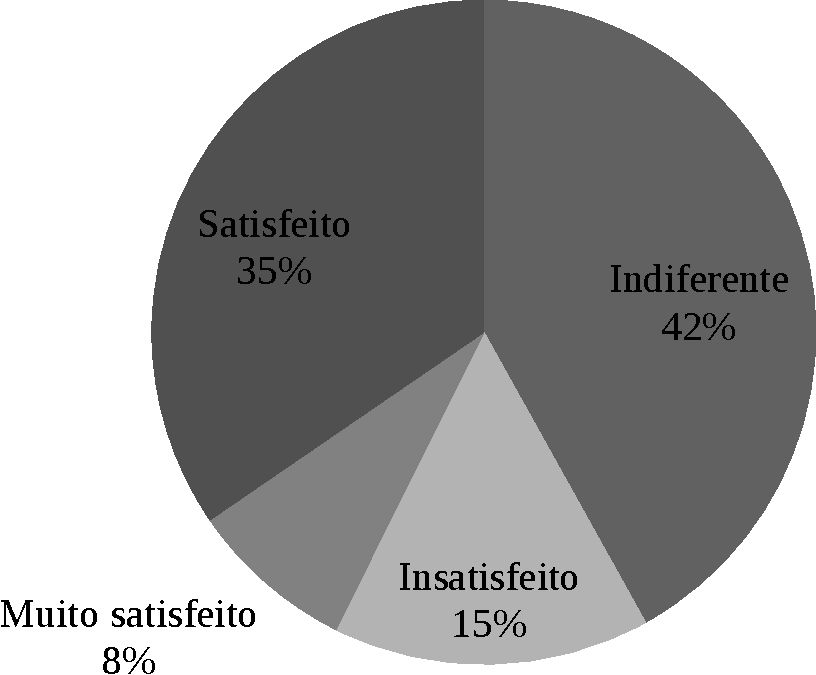
\includegraphics[width=0.55\linewidth]{plots/q17a.pdf}
	\captionof{figure}{Opinião dos alunos de \arat com mais\\de 28 anos pagando mensalidade via Financiamento\\Bancário.}
	\label{fig:opiniao-28anos-finBancario}
\end{minipage}
\end{figure}

\paragraph{(b)}

A Tabela \ref{table:opiniao-28anos-proprios} apresenta as frequências dos valores da variável \textit{Opinião} dos alunos que estão de \jaqu, com \textit{Idade} maior de 28 anos e Pagamento do tipo \textit{Recursos Próprios}. Os porcentuais desses valores podem ser observados no gráfico de setores da Figura \ref{fig:opiniao-28anos-proprios}.
Pode-se observar que a maioria, $53.66\%$ dos alunos, está insatisfeita, e incluindo os alunos muito insatisfeitos, obtém-se $60.98\%$ do total. Dos $39.02\%$ restantes, a maioria é de alunos indiferentes ($34.15\%$) e apenas dois alunos (4.88\%) declararam-se satisfeitos.

\begin{figure}[h]
\begin{minipage}{0.39\textwidth}
	\footnotesize
	\centering
	\captionof{table}{Frequência dos valores de \textit{Opinião} para alunos de \arat com mais de 28 anos pagando mensalidade via Financiamento Bancário.}
	\label{table:opiniao-28anos-proprios}
	\begin{tabular}{l r}
		\toprule
		\textbf{Opinião}    & \textbf{Frequência} \\
		\midrule
		Muito Insatisfeito  &  3  \\
		Insatisfeito        &  22 \\
		Indiferente         &  14 \\
		Satisfeito          &  2  \\
		\midrule
		Total               &  41 \\
		\bottomrule
	\end{tabular}
\end{minipage}
%
\begin{minipage}{0.69\textwidth}
	\centering
	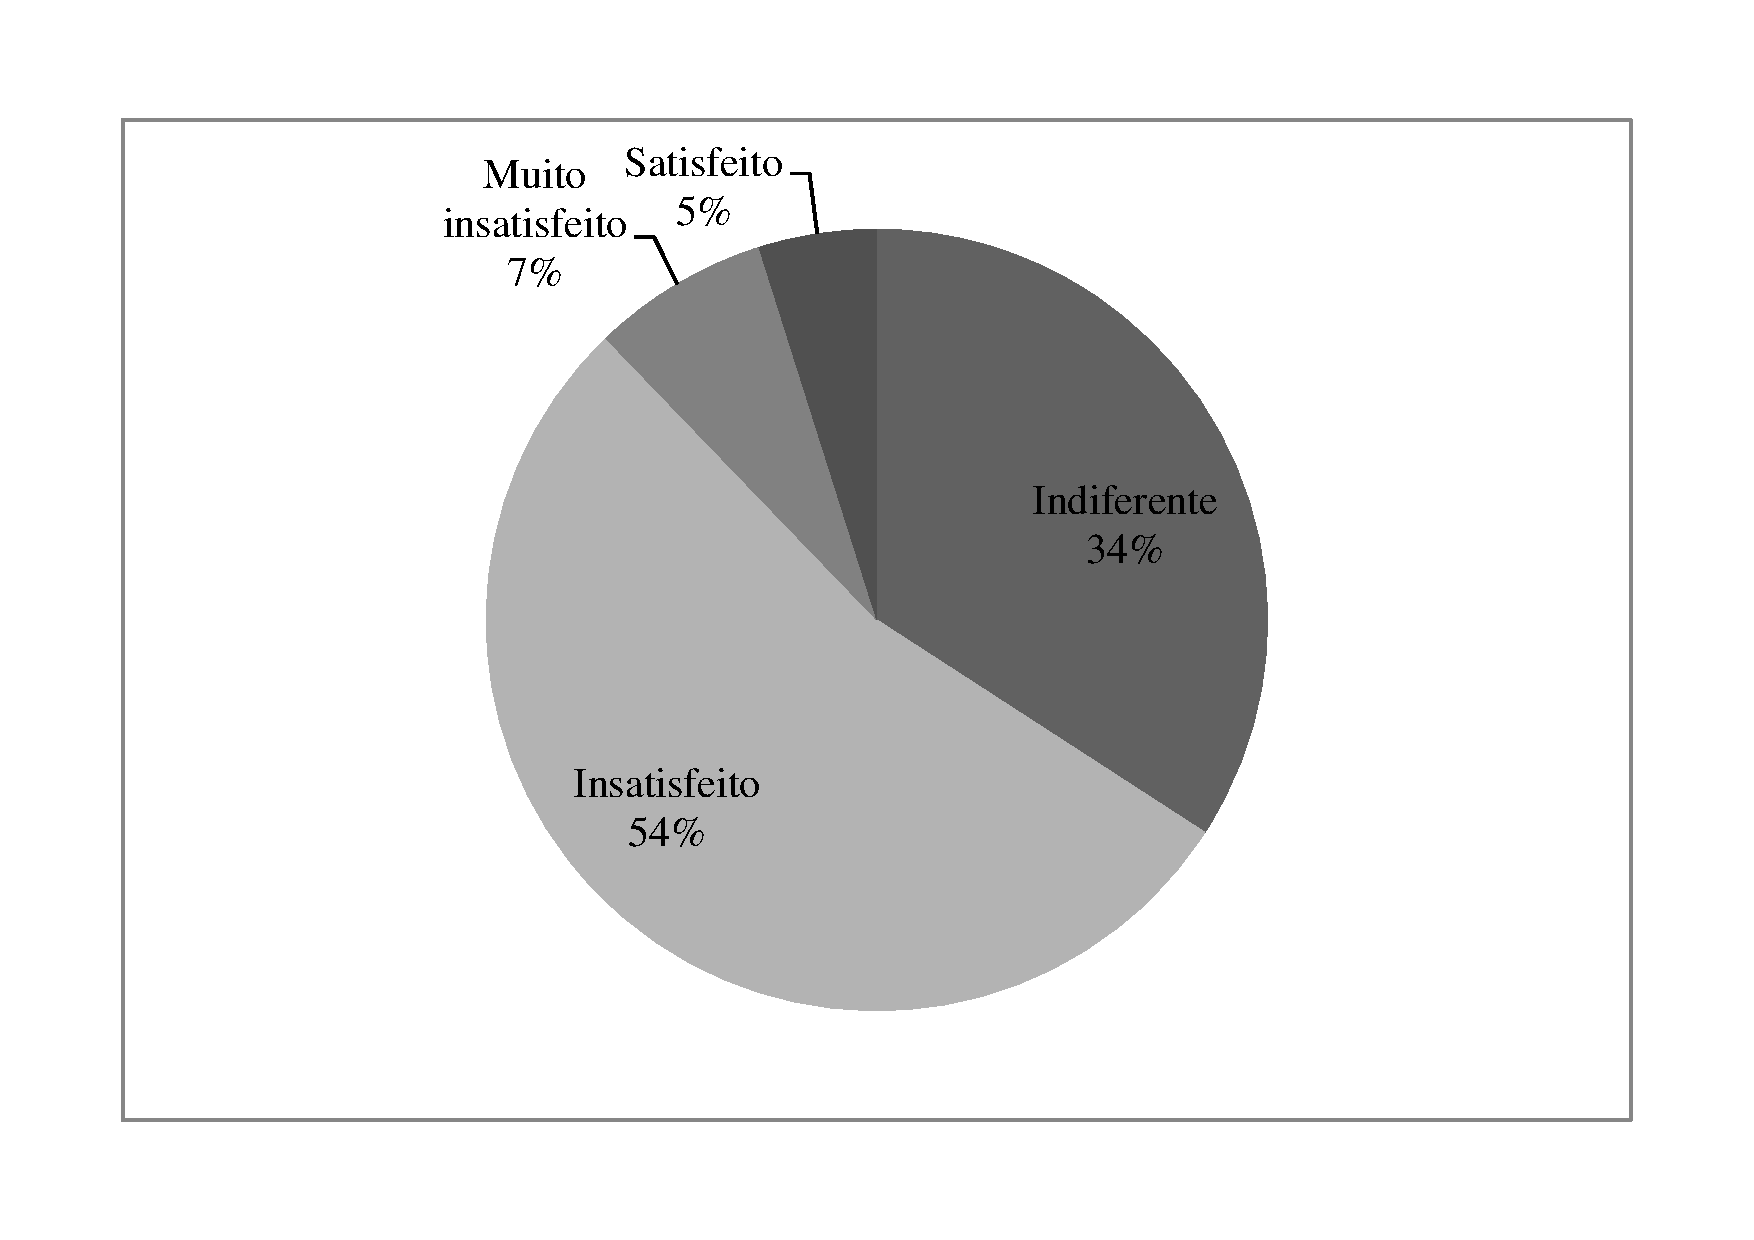
\includegraphics[width=0.55\linewidth]{plots/q17b.pdf}
	\captionof{figure}{Opinião dos alunos de \jaqu com mais\\de 28 anos pagando mensalidade com Recursos próprios.}
	\label{fig:opiniao-28anos-proprios}
\end{minipage}
\end{figure}

\paragraph{(c)}

A Tabela \ref{table:opiniao-28anos-incFederais} apresenta as frequências dos valores da variável \textit{Opinião} dentre os alunos que de \para, com mais de 28 anos e financiados por \textit{Incentivos Federais}. Uma representação desses valores é mostrada em um gráfico de setores na Figura \ref{fig:opiniao-28anos-incFederaiso}.
Pode-se observar que $92.24\%$ dos alunos estão muito insatisfeitos e $7.76\%$ estão insatisfeitos, não havendo, na amostra, dados de alunos indiferentes, satisfeitos ou insatisfeitos.
É possível notar que existe uma plena insatisfação por parte alunos acima de 28 anos da região \para e que recebem Incentivos federais.

\begin{figure}[h]
\begin{minipage}{0.39\textwidth}
	\footnotesize
	\centering
	\captionof{table}{Frequência dos valores de \textit{Opinião} para alunos de \arat com mais de 28 anos pagando mensalidade via Financiamento Bancário.}
	\label{table:opiniao-28anos-incFederais}
	\begin{tabular}{l r}
		\toprule
		\textbf{Opinião}    & \textbf{Frequência} \\
		\midrule
		Muito Insatisfeito  &  3  \\
		Insatisfeito        &  22 \\
		Indiferente         &  14 \\
		Satisfeito          &  2  \\
		\midrule
		Total               &  41 \\
		\bottomrule
	\end{tabular}
\end{minipage}
%
\begin{minipage}{0.69\textwidth}
	\centering
	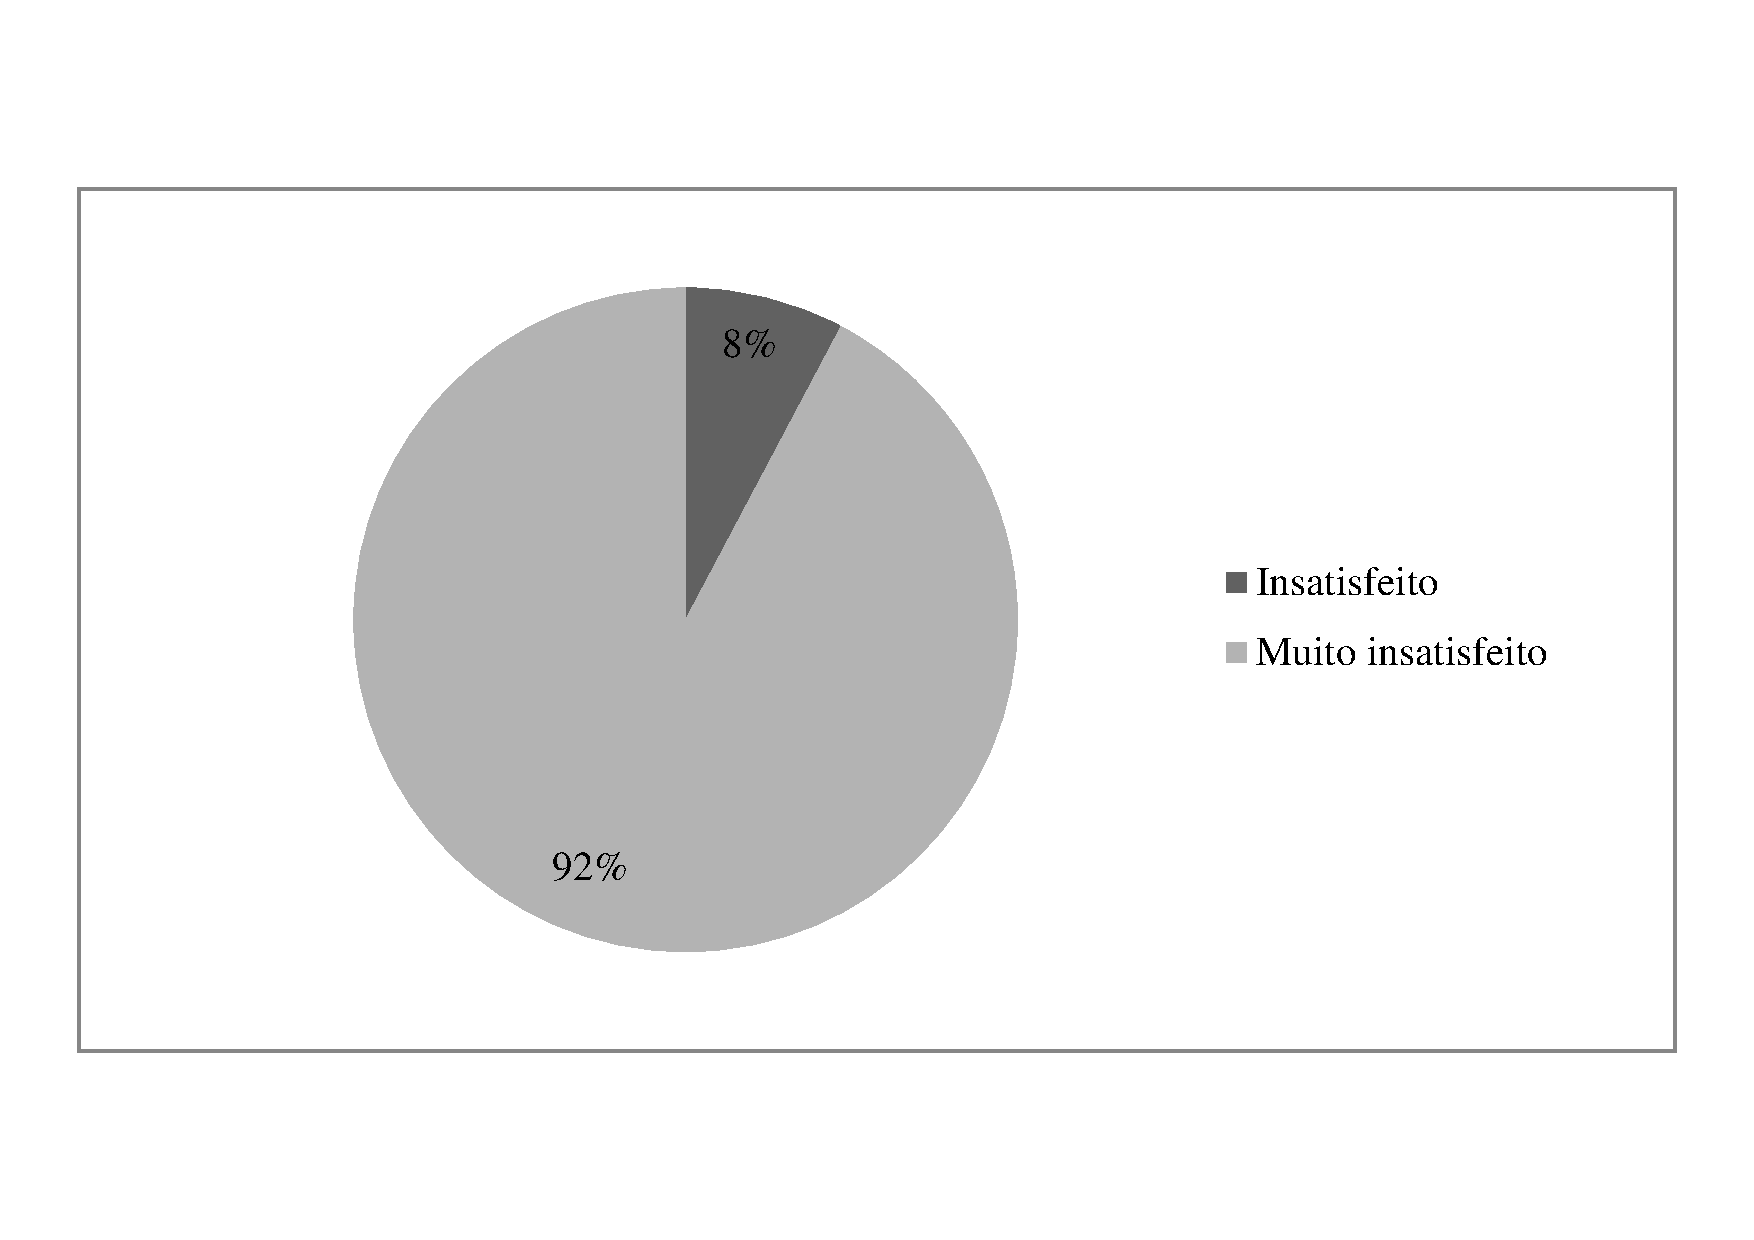
\includegraphics[width=0.70\linewidth]{plots/q17c.pdf}
	\caption{Opinião dos alunos de \para com mais\\de 28 anos pagando mensalidade via Incentivos Federais.}
	\label{fig:opiniao-28anos-incFederaiso}
\end{minipage}
\end{figure}

\FloatBarrier{}
\section{Recomendações para o Cliente: Outras variáveis}
\label{section:outras-variaveis}
Outras variáveis necessárias para caracterizar adequadamente a opinião dos alunos de EAD da TYU são  "Gênero" e "Rendimento do aluno" no curso.

% eu não concordo com algumas coisas que escrevi, não me odeiem
O Gênero tem sido uma variável popular e presente em diversos estudos disponíveis ao público. 
Amplo uso dessa variável tem sido feito nos mais diversos contextos com objetivo de encontrar correlações entre o gênero e outras variáveis. Essa busca por correlações frequentemente pode ser associada a verificação da desigualdade de gêneros. No caso da TYU, a verificação dessa desigualdade pode motivar políticas que a reduzam, e se verificada igualdade de gênero, os resultados podem ser usados em marketing. Podem ser estudadas, por exemplo, as seguintes relações:
\begin{itemize}
	\item Participação dos gêneros em cada região: Os alunos da TYU têm uma distribuição de gênero similar ao da população da região em estudo?
	\item Participação dos gêneros por área: Como a TYU se compara nesse aspecto com outras universidades ou com os totais nacionais de Pindorama? A TYU é mais inclusiva ou ou há espaço para melhora?
	\item Distribuição da Opinião por gênero: Algum gênero está particularmente insatisfeito? Possíveis alterações podem ser estudadas para melhorar a opinião e/ou prevenir a evasão nos cursos;
	\item Participação de gênero em incentivos federais e bolsas de estudo: Essas modalidades de auxílio possuem viés a um gênero?
\end{itemize}

O rendimento acadêmico do aluno pode ser usado para identificar a necessidade de mudanças na área pedagógica dos cursos e dos polos de EAD. Inclusive, nos dados analisados neste relatório, foram incluídos apenas alunos com rendimento acadêmico superior a 5 - isso tende a ser uma possível fonte de erros. Os alunos com rendimento inferior, ainda assim são alunos da TYU e a sua ausência na amostra pode ter enviesado os resultados, fazendo com que futuras ações de melhorias tomadas pela direção da TYU não levem em consideração esse grupo de alunos, possivelmente ocasionando uma maior evasão entre os alunos nesse grupo. Como o rendimento é uma medida particular da TYU, não é confiável realizar sua comparação com índices de outras instituições. Entretanto, assim como no caso do gênero, diversas análises em conjunto com as outras variáveis são possíveis:
\begin{itemize}
	\item Qual é a distribuição do rendimento dado um dos valores de Opinião? Por exemplo, alunos insatisfeitos com rendimento alto pode ser um indicativo de ensino e avaliação pedagógica mais frouxos.
	\item Qual a distribuição do rendimento em cada área em cada região? Quais cursos em quais polos precisam de mais atenção em relação aos tutores e professores? Tal análise poderia guiar o investimento em laboratórios, além quando da contratação de tutores e docentes;
	\item Qual a distribuição do rendimento por fonte de pagamento? Alunos contemplados com Bolsas ou incentivos federais estão apresentando desempenho acadêmico superior aos seus pares que possuem outros tipos de financiamento? 
	\item Qual a distribuição do rendimento por renda? Alunos pobres conseguem manter um rendimento acadêmico similar aos demais grupos de renda? Refinando essa análise aplicando agrupamentos por fonte de pagamento, seria possível identificar grupos de alunos de acordo com renda e fonte de pagamento que precisem de atenção pedagógica especial.
\end{itemize}

\FloatBarrier
\section{Recomendação para o Cliente: Sugestão de Análises}
\label{section:sugestao}

Uma análise que poderia ser feita é a relação entre \textit{Renda}, \textit{Área} e \textit{Opinião}. Assim seria possível complementar a análise da Seção \ref{section:opiniao-area} verificando se a área com alunos mais insatisfeitos está relacionada com alunos mais abastados.

Uma segunda análise seria a relação entre \textit{Área} e \textit{Pagamento}. Tal análise permite avaliar a opinião dos alunos de acordo com a forma de pagamento e a sua área cursada. Em outras palavras, seria 
possível verificar se a forma de pagamento predominante de cada área está relacionada com a opinião dos alunos.

\FloatBarrier
\section{Recomendação para o Cliente: Análises Sugeridas}
\label{section:analises}

\paragraph{a}{\textbf{Área x Renda x Opinião}}

Com a análise das Tabelas \ref{tab:q20} e \ref{tab:q20p} é possível observar que na área da \adm os alunos mais abastados estão mais insatisfeitos ($44.44\%$), seguido por 
indiferentes (37.04\%). Os intermediários são mais satisfeitos ($46.71\%$) e muito satisfeitos ($33.54\%$), enquanto os pobres estão muito satisfeitos ($92.53\%$) e satisfeitos ($7.05\%$).

% latex table generated in R 3.2.4 by xtable 1.8-2 package
% Mon Apr 11 15:32:41 2016
\begin{table}[ht]
\scriptsize
\centering
\begin{tabular}{ll rrrrr}
  \toprule
 Área                    & Classe $\vert$ Opinião & \multicolumn{1}{l}{ Muito insatisfeito} & \multicolumn{1}{l}{ Insatisfeito} & \multicolumn{1}{l}{ Indiferente} & \multicolumn{1}{l}{ Satisfeito} & \multicolumn{1}{l}{ Muito satisfeito} \\ 
   \midrule
Administração           & Abastados               &                  1 &           12 &          10 &          3 &                1 \\ 
                          & Intermediario           &                  1 &            9 &          53 &        149 &              107 \\ 
                          & Pobres                  &                  0 &            0 &           1 &         17 &              223 \\ 
  Computação e Matemática & Abastados               &                  2 &            7 &           9 &          6 &                2 \\ 
                          & Intermediario           &                  0 &            8 &          45 &         77 &               58 \\ 
                          & Pobres                  &                  0 &            0 &           2 &          8 &               71 \\ 
  Educacional             & Abastados               &                  0 &            1 &           0 &          0 &                4 \\ 
                          & Intermediario           &                  0 &            1 &           6 &         22 &               30 \\ 
                          & Pobres                  &                  0 &            0 &           0 &          4 &              269 \\ 
  Engenharia e Produção   & Abastados               &                 64 &          154 &         104 &         23 &                2 \\ 
                          & Intermediario           &                  4 &           92 &         376 &        389 &              219 \\ 
                          & Pobres                  &                  0 &            0 &           2 &         50 &              248 \\ 
  Humanidades             & Abastados               &                  0 &            4 &           7 &          2 &                3 \\ 
                          & Intermediario           &                  0 &            4 &          27 &         73 &               87 \\ 
                          & Pobres                  &                  0 &            0 &           0 &          8 &              284 \\ 
  Jurídica e Contábil     & Abastados               &                391 &          331 &          90 &          9 &                0 \\ 
                          & Intermediario           &                  7 &          123 &         263 &        174 &               60 \\ 
                          & Pobres                  &                  0 &            0 &           1 &         15 &               37 \\ 
   \bottomrule
\end{tabular}
\end{table}


% latex table generated in R 3.2.4 by xtable 1.8-2 package
% Mon Apr 11 14:59:08 2016
\begin{table}[h]
\scriptsize
\centering
\label{tabela:q20p}
\begin{tabular}{ll rrrrr}
  \toprule
\textbf{Região}    & \textbf{Classe}  & \textbf{\specialcell{c}{Muito\\insatisfeito}} & \textbf{Insatisfeito} & \textbf{Indiferente} & \textbf{Satisfeito} & \textbf{\specialcell{c}{Muito\\satisfeito}}\\ 
   \midrule
Aratibutantã  & Abastados               &              19.88 &        51.77 &       25.00 &       3.15 &             0.20 \\ 
                & Intermediario           &               0.90 &        17.77 &       49.40 &      25.90 &             6.02 \\ 
                & Pobres                  &               0.00 &         0.00 &        0.00 &      50.00 &            50.00 \\ 
\midrule
  Baependinha   & Abastados               &               7.10 &        37.42 &       34.84 &      16.13 &             4.52 \\ 
                & Intermediario           &               0.25 &         5.22 &       25.34 &      41.49 &            27.70 \\ 
                & Pobres                  &               0.00 &         0.00 &        0.98 &      16.54 &            82.48 \\ 
\midrule
     Itamaracanã   & Abastados               &               0.00 &         0.00 &        0.00 &       0.00 &           100.00 \\ 
                & Intermediario           &               0.00 &         0.00 &        5.45 &      27.27 &            67.27 \\ 
                & Pobres                  &               0.00 &         0.00 &        0.14 &       1.93 &            97.93 \\ 
\midrule
     Jaquereçaba   & Abastados               &              51.32 &        39.04 &        8.99 &       0.66 &             0.00 \\ 
                & Intermediario           &               2.60 &        45.45 &       40.26 &      11.69 &             0.00 \\ 
                & Pobres                  &               0.00 &         0.00 &        0.00 &       0.00 &             0.00 \\ 
\midrule
     Paranapitanga & Abastados               &              91.74 &         8.26 &        0.00 &       0.00 &             0.00 \\ 
                & Intermediario           &               0.00 &         0.00 &        0.00 &       0.00 &             0.00 \\ 
                & Pobres                  &               0.00 &         0.00 &        0.00 &       0.00 &             0.00 \\ 
\bottomrule
\end{tabular}
\end{table}



Na área da \comp, os mais abastados são indiferentes (34.62\%) e insatisfeitos (26.92\%). Já os intermediários são mais satisfeitos (40.96\%) e muito satisfeito (30.85\%) e 
os pobres são muito satisfeitos (87.65\%) e satisfeitos (9.88\%).

Na área da \edu os abastados são muito satisfeitos ($80\%$) e insatisfeitos ($20\%$). Já os intermediários são muito satisfeitos ($50.85\%$) e satisfeitos ($37.29\%$) e os pobres são muito 
satisfeitos ($98.53\%$) e satisfeitos ($1.47\%$).

A área da \eng apresenta índices de insatisfeitos ($44.38\%$) e indiferentes ($29.97\%$) para os abastados, enquanto satisfeitos ($36.02\%$) e indiferentes ($34.81\%$) representam os intermediários.
Já os pobres, estão muito satisfeitos ($82.67\%$) e satisfeitos ($16.67\%$).

Na área da \hum os abastados são indiferentes ($43.75\%$) e insatisfeitos ($25\%$), os intermediários são muito satisfeitos ($45.55\%$) e satisfeitos ($38.22\%$) e os pobres são muito 
satisfeitos ($97.26\%$) e satisfeitos ($2.74\%$).

Por fim, na área \jur os abastados são muito insatisfeitos ($47.62\%$) e insatisfeitos ($40.32\%$), os intermediários são indiferentes (41.95\%) e satisfeitos ($27.75\%$) e os 
pobres são muito satisfeitos ($69.81\%$) e satisfeitos ($28.30\%$).

Ao analisar as Tabelas \ref{tab:q20} e \ref{tab:q20p}, pode-se inferir que os alunos de classes mais pobres estão muito satisfeitos ou satisfeitos. Já os abastados estão mais insatisfeitos, enquanto os 
intermediários variam de opinião de acordo com o curso.

\paragraph{b}{\textbf{Área x Pagamento}}

Analisando as Tabelas \ref{table:area-pag-abs} e \ref{table:area-pag-rel} pode-se observar que a forma de pagamento mais utilizada pelos alunos da universidade TYU é por Financiamento Bancário ($43.94\%$), seguida por incentivos federais ($29.11\%$) e Recursos Próprios ($15.22\%$), ficando com os menores índices as Bolsas de Estudos ($6.55\%$) e Auxílio de Familiares ($5.18\%$). Estas informações também podem ser analisadas pelo gráfico de barras ilustrado na Figura \ref{fig:q20b}.

\begin{table}[h]
\scriptsize
\centering
\caption{Relação entre as variáveis Área e Pagamento usando valores absolutos}
\label{table:area-pag-abs}
\begin{tabular}{l rrrrrr}
\toprule
\textbf{Área}    & \textbf{\specialcell{c}{Auxílio de\\ familiares}} & \textbf{\specialcell{c}{Bolsas de\\ estudos}} & \textbf{\specialcell{c}{Financiamento\\ bancário}} & \textbf{\specialcell{c}{Incentivos\\ federais}} & \textbf{\specialcell{c}{Recursos\\ próprios}} & 
\textbf{Total} \\
\midrule
Administração  &  18 & 28 & 401 & 60 & 83 & \textbf{590}  \\
Computação e Matemática        &  15 & 19 & 162 & 37 & 63 & \textbf{296} \\
Educacional         &  3 & 5 & 310 & 4 & 16 & \textbf{338} \\
Engenharia e Produção          &  113 & 134 & 683 & 464 & 339 & \textbf{1733}  \\
Humanidades & 17 & 11 & 392 & 21 & 61 & \textbf{502} \\
Jurídica e Contábil & 91 & 128 & 232 & 858 & 193 & \textbf{1502} \\
\midrule
\textbf{Total} &  \textbf{257} &\textbf{325} & \textbf{2180} & \textbf{1444} & \textbf{755} & \textbf{4961} \\
\bottomrule
\end{tabular}
\end{table}

\begin{table}[h]
\scriptsize
\centering
\caption{Relação entre as variáveis \textbf{Área} e \textbf{Pagamento} usando valores relativos}
\label{table:area-pag-rel}
\begin{tabular}{l rrrrr}
\toprule
\textbf{Área}    & \textbf{\specialcell{c}{Auxílio de\\ familiares}} & \textbf{\specialcell{c}{Bolsas de\\ estudos}} & \textbf{\specialcell{c}{Financiamento\\ bancário}} & 
\textbf{\specialcell{c}{Incentivos\\ federais}} & \textbf{\specialcell{c}{Recursos\\ próprios}} \\%& \textbf{Total} \\
\midrule
Administração  			&  $3.05\%$ &  $4.75\%$ &  $67.97\%$ &  $10.17\%$ &  $14.07\%$ \\%&  \textbf{100.00\%}  \\
Computação e Matemática &  $5.07\%$ &  $6.42\%$ &  $54.73\%$ &  $12.50\%$ &  $21.28\%$ \\%&  \textbf{100.00\%} \\
Educacional         	&  $0.89\%$ &  $1.48\%$ &  $91.72\%$ &  $1.18\%$  &  $4.73\%$ \\%&  \textbf{100.00\%} \\
Engenharia e Produção   &  $6.52\%$ &  $7.73\%$ &  $39.41\%$ &  $26.77\%$ &  $19.56\%$ \\%&  \textbf{100.00\%}  \\
Humanidades 			&  $3.39\%$ &  $2.19\%$ &  $78.09\%$ &  $4.18\%$  &  $12.15\%$ \\%&  \textbf{100.00\%} \\
Jurídica e Contábil 	&  $6.06\%$ &  $8.52\%$ &  $15.45\%$ &  $57.12\%$ &  $12.85\%$ \\%&  \textbf{100.00\%} \\
%\midrule
%\textbf{Total}          &  \textbf{5.18\%} &  \textbf{6.55\%} &  \textbf{43.94\%} &  \textbf{29.11\%} &  \textbf{15.22\%} &  \textbf{100.00\%} \\
\bottomrule
\end{tabular}
\end{table}

As áreas que utilizam predominantemente a forma de pagamento por Financiamento Bancário é a \edu ($91.72\%$), seguida pela \hum ($78.09\%$) e \adm ($67.97\%$), ficando com índices mais baixos as áreas \comp ($54.73\%$), \eng ($39.41\%$) e \jur ($15.45\%$). Já a opinião com  maiores índices dos alunos que utilizam o financiamento bancário como forma de pagamento, conforme apresentada na Tabela \ref{table: avaliacao por fonte de pagamento-percent}, é muito satisfeito ($66.09\%$) e satisfeito ($22.68\%$). Tal análise pode ser confirmada com a Tabela \ref{table:opiniao-por-area}, pois os alunos das áreas \edu ($89.91\%$), \hum ($74.90\%$) e \adm ($56.37\%$) possuem maiores níveis de satisfação.

Os alunos da área \jur, predominantemente pagam suas mensalidades com recursos de Incentivos Federais ($57.12\%$). Conforme apresentado na Tabela \ref{table:opiniao-por-area}, os alunos da área 
\jur estão mais insatisfeitos ($30.17\%$) e muito insatisfeitos ($26.45\%$). Os resultados da Tabela \ref{table: avaliacao por fonte de pagamento} mostram que os alunos que pagam suas mensalidades com incentivos federais são 
mais insatisfeitos (35.15\%) e muito insatisfeitos ($39.77\%$). De acordo com essas observações pode-se ratificar, através da análise das Tabelas \ref{table:area-pag-abs} e \ref{table:area-pag-rel}, que 
os alunos da área \jur são mais insatisfeitos.

\begin{figure}[ht]
	\centering
	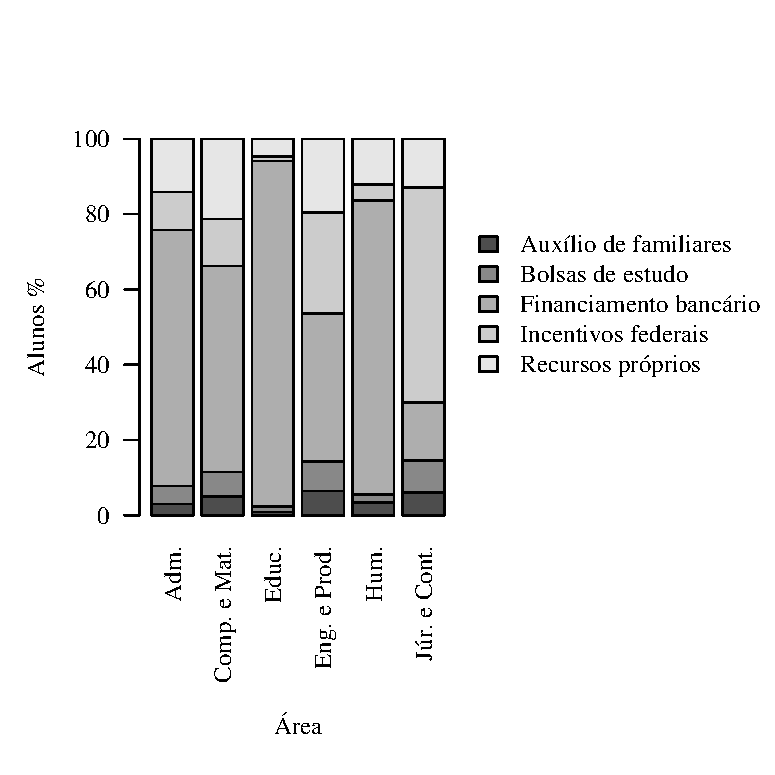
\includegraphics[width=0.70\linewidth]{plots/stacked100_pagamento_por_area.eps}
	\caption{Gráfico de barras empilhadas mostrando a proporção dos tipos de pagamento para cada área.}
	\label{fig:q20b}
\end{figure}

Já a forma de pagamento por recursos próprios tem predominância nas áreas \comp ($21.28\%$), \eng ($19.56\%$), \adm ($14.07\%$), \jur($12.85\%$) e \hum ($12.15\%$). A análise da Tabela \ref{table: avaliacao por fonte de pagamento} mostra que os alunos que pagam suas mensalidades com esta forma de pagamento são mais indiferentes ($31.40\%$) e satisfeitos ($21.90\%$). 

A forma de pagamento com bolsa de estudo apresenta com predominância nas áreas \jur ($8.52\%$), \eng ($7.73\%$), \comp ($6.42\%$), \adm ($4.75\%$), \hum ($2.19\%$) e \edu($1.48\%$). Segundo a análise da Tabela \ref{table: avaliacao por fonte de pagamento} alunos que pagam suas mensalidades com essa forma de pagamento 
são mais indiferentes ($38.72\%$) e satisfeitos ($22.87\%$).

Por fim, a forma de pagamento por auxílio de familiares é predominante para as áreas \eng($6.52\%$), \jur ($6.06\%$), \comp ($5.07\%$), \hum($3.39\%$), \adm ($3.05\%$) e \edu ($0.89\%$). A Tabela \ref{table: avaliacao por fonte de pagamento} aponta ainda que alunos que pagam suas mensalidades com essa forma de pagamento são mais indiferentes ($36.96\%$) e satisfeitos ($30.35\%$).

\end{document}
